\documentclass[a4paper]{article}
\usepackage{Sweave}
\usepackage{longtable}
\usepackage{caption}
\usepackage{tabularx}
\usepackage{ltxtable}
\usepackage{hyperref}
\usepackage{fancyhdr}
\usepackage[utf8]{inputenc}
\usepackage[top=.75in, bottom=1in, left=1in, right=1in]{geometry}


\title{Alveolar Fricative Voicing in Appalachia: Preliminary Investigation}
\author{Doug Raffle\\STAT 695}
\date{\today}

\begin{document}
\vspace{-30pt}
\maketitle
\tableofcontents
\thispagestyle{empty}

\newpage
\setcounter{page}{1}
\pagestyle{fancy}
\fancyhead{}
\fancyfoot{}
\fancyhead[R]{Doug Raffle}
\fancyhead[L]{\bf Alveolar Fricative Voicing in Appalacia}
\fancyfoot[LE, RO]{\thepage}
\section*{Background}
\addcontentsline{toc}{section}{Background}
The goal of this study is to identify which sociolinguistic
variables are most associated with how speakers of the Appalachian
Dialect voice alveolar fricatives.  Fricatives are consonants
that are produced by forcing air between two articulators, in this
case the tongue and alveolar ridge (which is the ridge in your mouth
between your upper teeth and the hard palate at the top of your
mouth).  A sibilant is a consonant where the tongue is curled so that
the air also flows under the edge of the teeth; alveolar
fricatives are a subset of this class.  Like most consonant classes,
alveolar fricatives can be voiced or voiceless.  Voiced alveolar
fricatives are [z] sounds, and voiceless alveolar fricatives are [s]
sounds.

The simplest explanation of voicing is whether or not the vocal
chords vibrate (referred to as glottal pulsing) as a sound is
produced.  However, recent studies in psycholinguistics have revealed that the
perception of voicing is actually a very complicated phenomenon,
and whether a listener perceives a sound as voiced or voiceless depends
on several variables.  A change in any one of these variables can
change this perception.
Because of this, studying voicing cannot simply be done by
categorizing a sound a ``voiced'' or ``voiceless,'' as convenient as
that might be.  In this study,
the four main variables that are being considered as
indicative of voicing are the Duration of the Sibilant, Center of
Gravity, Percent Voicelessness of the sibilant, and the Duration of
the Preceding Segment\footnote{
  For a full listing of variables and their definitions,
  see Appendix \ref{a:vardef}
}$^,$\footnote{I'll try to get references for these studies from Dr. Hazen
  at some point.
}

Simply put, this study is concerned with whether speakers pronounce
the ``s'' in a word like ``brothers'' with an [s] sound like in
``bus'' (voiceless), or a [z] sound as in ``buzz'' (voiced), and, perhaps more
importantly, it is about how we quantify that difference.

\section*{Data Collection}
\addcontentsline{toc}{section}{Data Collection}
Sixty-seven interviews were conducted with life-long residents of
the Appalachian Region of the United States, including West Virginia,
Southwestern Pennsylvania, and Southeastern Ohio.  Demographic
information was recorded for each speaker.  Tokens, which are
the unique speech acts that make up the observations in the data,
containing alveolar fricatives were identified in audio recordings of the
interviews and analyzed using Praat\footnote{
  Praat is a software suite purpose built for analyzing phonetic data.\\
  \url{http://www.fon.hum.uva.nl/praat/}
}.  There are an average of forty-six tokens per speaker, with as few
as twenty-seven and as many as fifty-six (Figure \ref{fig:token_count}).
\vspace{-30pt}
\begin{figure}[ht]
  \begin{center}
    \begin{minipage}[t]{0.8\linewidth}
      \begin{center}
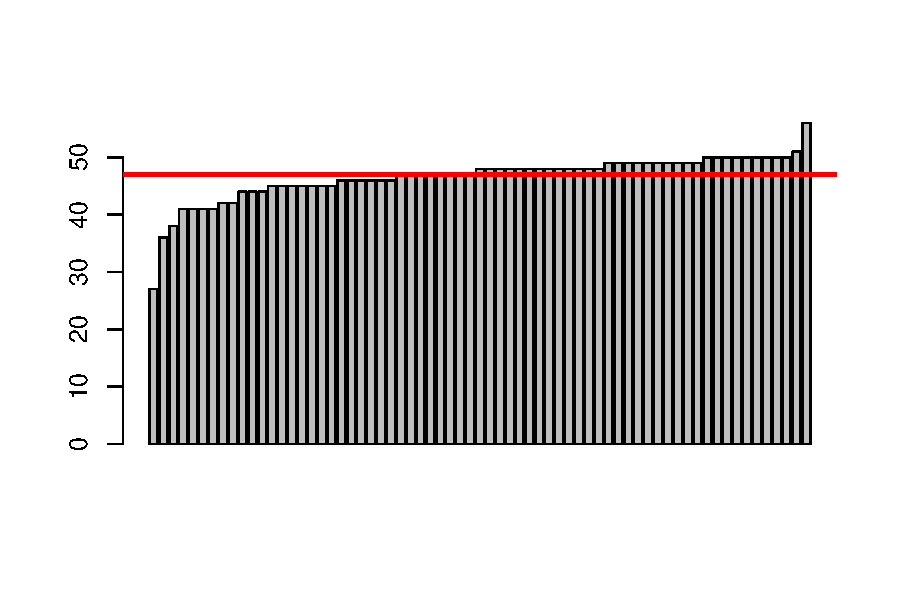
\includegraphics{prelim-003}
      \end{center}
    \end{minipage}
  \end{center}
  \vspace{-60pt}
  \caption{Token Count by Speaker}
  \label{fig:token_count}
\end{figure}
\section*{Independent Variables}
\addcontentsline{toc}{section}{Independent Variables}
\subsection*{Social Variables}
\addcontentsline{toc}{subsection}{Social Variables}
For each interviewee (speaker), researchers recorded their ethnicity,
education level, region, age, sex, social class, and rurality.  Most
of these variables are factors with two or three levels, but age is
recorded both as a numeric age in years and as a factor with four levels based on
age group.  While effort was made to find at least one token for every
combination of factor levels, there is substantial unbalance both the
number of tokens for each factor (Figure \ref{fig:social_by_token}) and
number of speakers for each factor (Figure
\ref{fig:social_by_speaker}), especially for \texttt{ethnicity},
\texttt{college}, \texttt{rurality}, and \texttt{class}.\\
\vspace{-5pt}
\begin{figure}[ht]
  \vspace{-5pt}
  \begin{center}
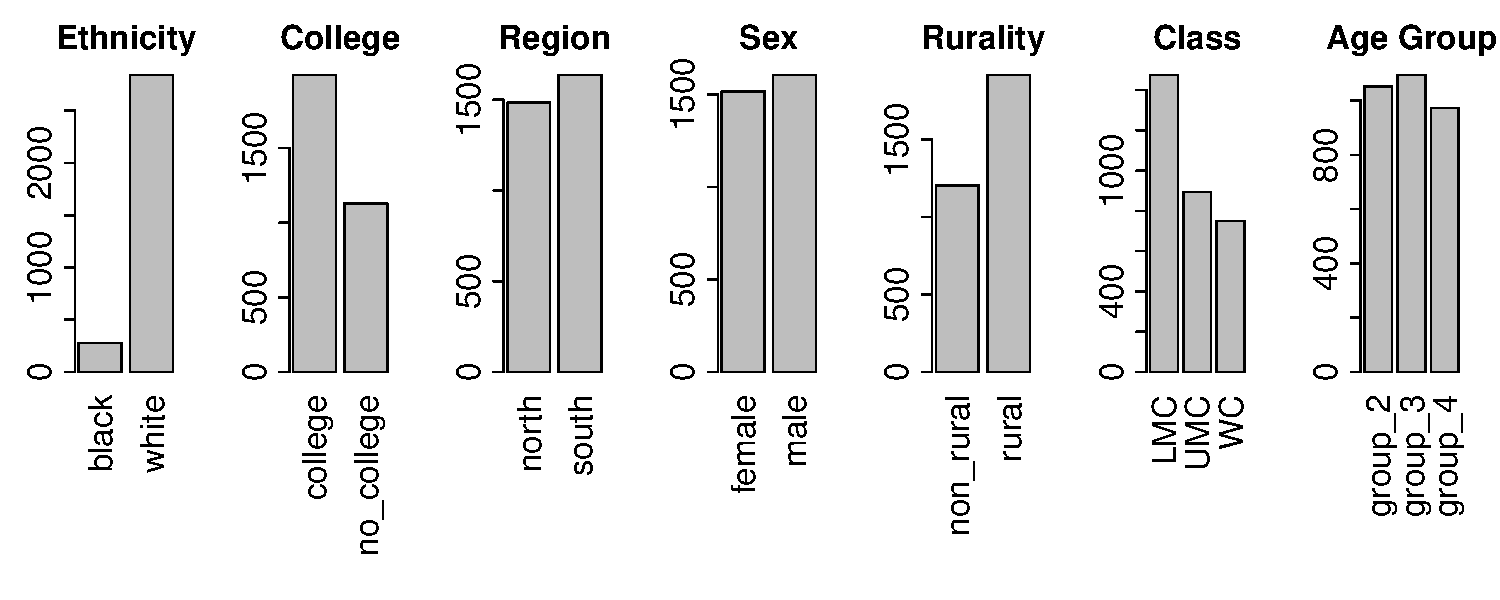
\includegraphics{prelim-005}
  \end{center}
  \vspace{-20pt}
  \caption{Token Counts by Social Variable}
  \label{fig:social_by_token}
\end{figure}

\begin{figure}[ht]
  \begin{center}
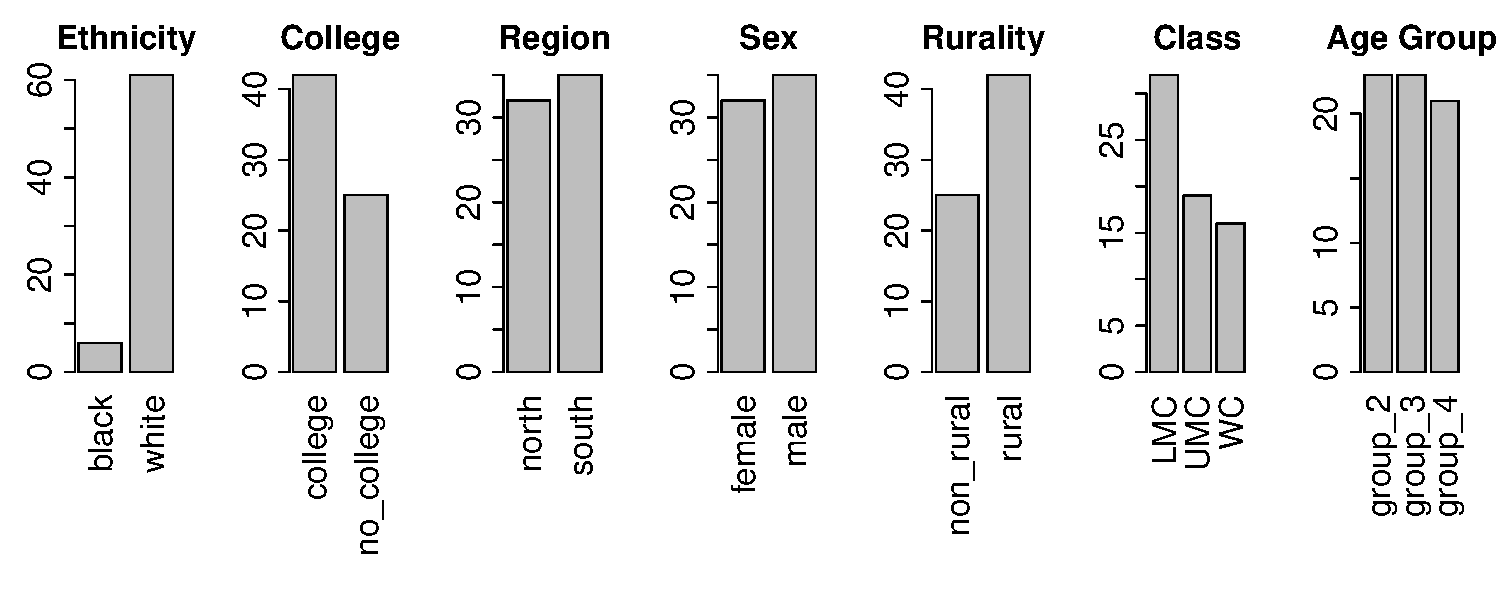
\includegraphics{prelim-007}
  \end{center}
  \vspace{-20pt}
  \caption{Speaker Counts by Social Variable}
  \label{fig:social_by_speaker}
\end{figure}
\newpage
While the age groups are fairly evenly represented, this is because
the age groups are not defined with even age ranges (see Appendex
\ref{a:vardef}).  When numeric ages are considered, it is obvious that
people between the ages of twenty and twenty-five far outnumber any
other similarly sized age range in the data (Figure
\ref{fig:age_by_speaker}).  Because of this, and the fact that both
age variables are collected at the speaker level and not at the token
level, it will probably be better to use \texttt{age\_group} as a factor
than \texttt{age} as a numeric predictor.\vspace{-10pt}

\begin{figure}[ht]
  \begin{center}
    \begin{minipage}[t]{0.35\linewidth}\begin{center}
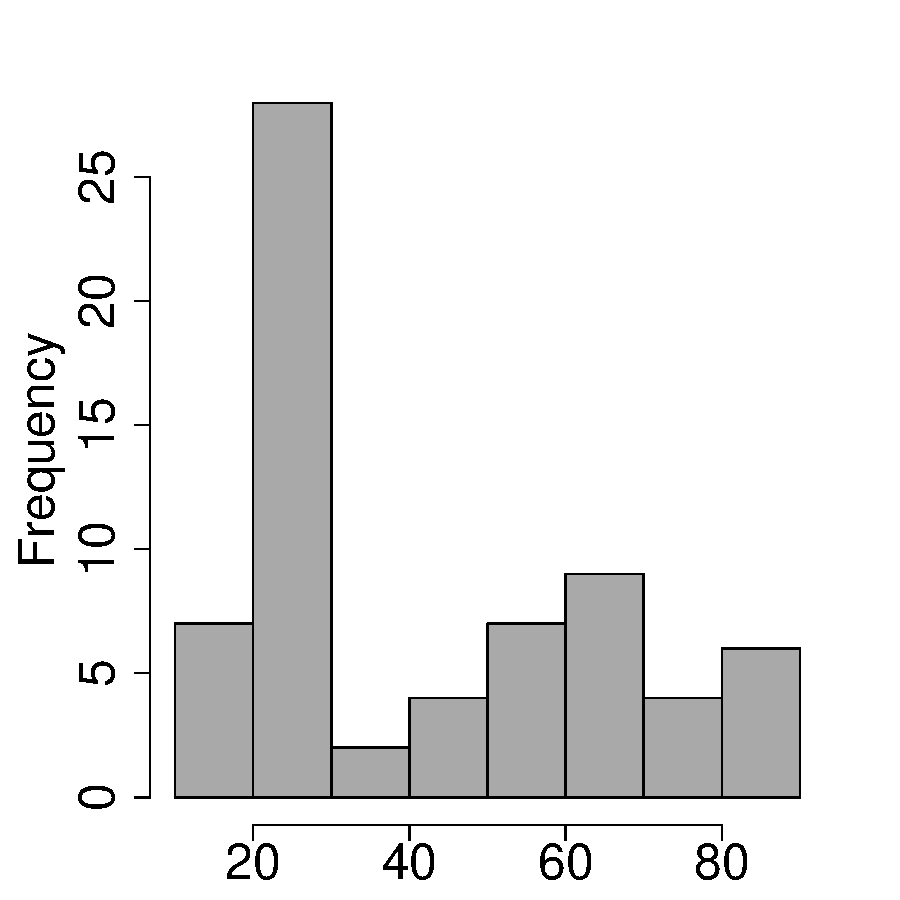
\includegraphics{prelim-009}
    \end{center}\end{minipage}
    \vspace{-5pt}
  \caption{Histogram of Speaker Ages}
  \label{fig:age_by_speaker}
  \end{center}
\end{figure}

\subsection*{Linguistic Variables}
\addcontentsline{toc}{subsection}{Linguistic Variables}
The linguistic variables were collected at the word or token level,
and describe the sibilant of interest and its linguistic environment.

\subsubsection*{Morphological Variables}
\addcontentsline{toc}{subsubsection}{Morphological Variables}
The morphological variables are both categorical variables.
Morphological Standing specifies how the word containing the sibilant
is stressed, and Sibilant Location describes where in that word the
sibilant occurs.   Almost all of the
sibilants are part of words that with primary or secondary stress in
the sentence, and there are many more word-final sibilants than
internal sibilants.\vspace{-5pt}

\begin{figure}[ht]
    \begin{center}
      \begin{minipage}[t]{0.3\linewidth}
        \begin{center}
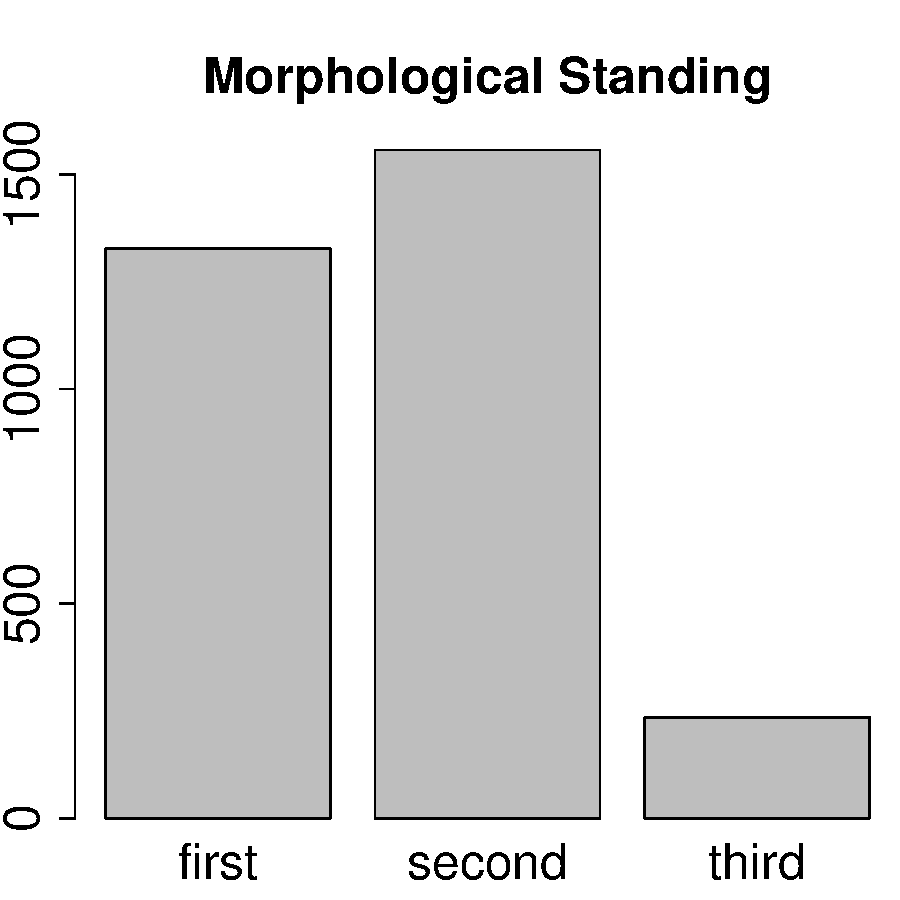
\includegraphics{prelim-012}
        \end{center}
      \end{minipage}
      \begin{minipage}[t]{0.3\linewidth}\begin{center}
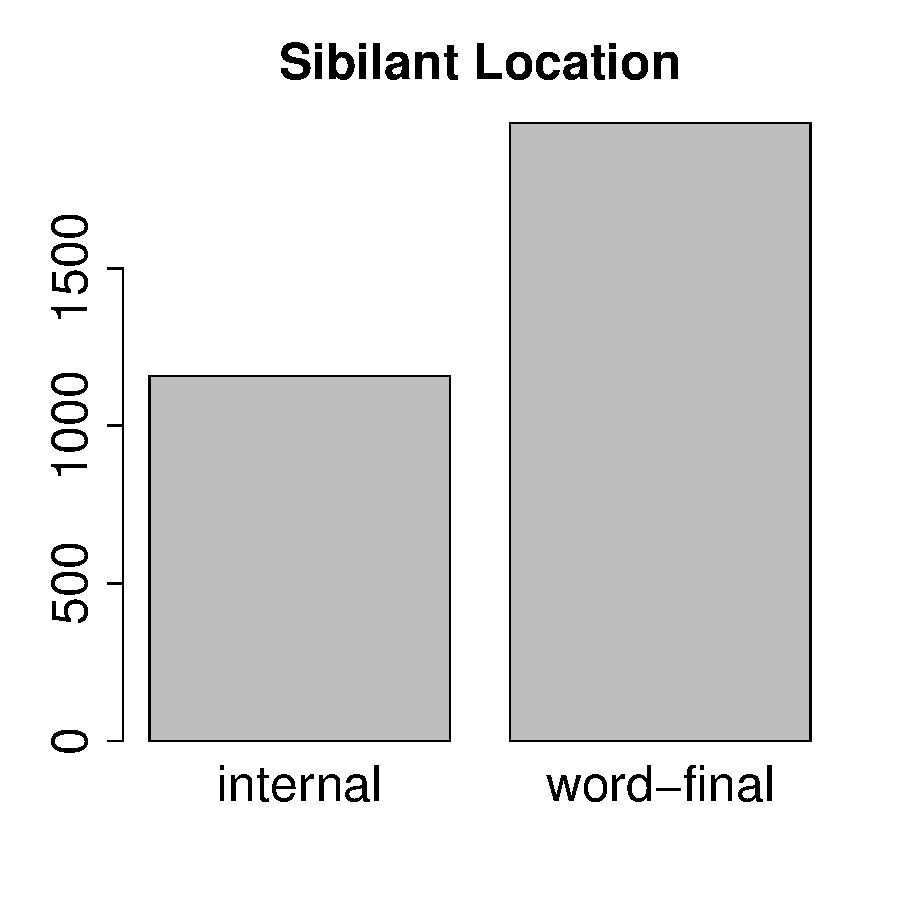
\includegraphics{prelim-013}
      \end{center}\end{minipage}
      \vspace{-5pt}
      \caption{Token Count by Morphological Variable}
      \label{fig:morpho}
    \end{center}
\end{figure}

\vspace{-20pt}
\subsection*{Phonological Variables}
\addcontentsline{toc}{subsubsection}{Phonological Variables}
The phonological variables describe the types of sounds that
precede and follow the sibilant, as well as its standard
pronunciation.  These variables are more closely associated with the word
than the token, but in the case where a pause follows a word-final
sibilant this line is blurred.\vspace{-5pt}


\begin{figure}[ht]
  \begin{center}
    \begin{minipage}[t]{0.8\linewidth}
      \begin{center}
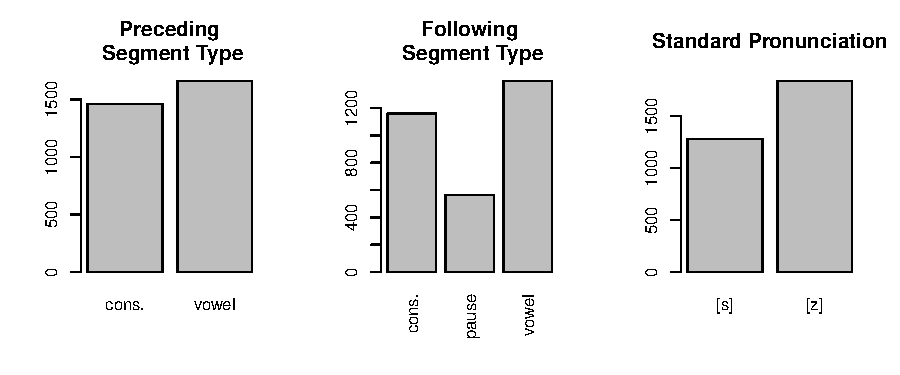
\includegraphics{prelim-015}
      \end{center}
    \end{minipage}
    \caption{Token Count by Phonological Variable}
    \label{fig:phono}
  \end{center}
\end{figure}
\subsection*{Phonetic Variables}
\addcontentsline{toc}{subsubsection}{Phonetic Variables}
The phonetic variables are physical characteristics of the
sibilant and the preceding segment, and they are collected at the
token level.  Pitch and intensity were measured
at three points in both the preceding segment and sibilant: at 5\%,
25\%, and 50\% through the duration of the sounds.\vspace{-15pt}

\begin{figure}[h]
  \begin{center}
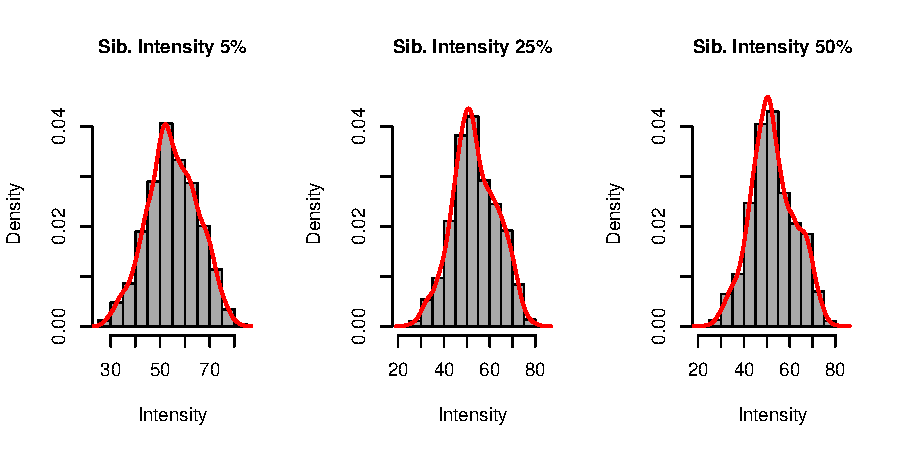
\includegraphics{prelim-017}
  \caption{Density Histograms of Sibilant Intensities}
  \label{fig:sib.intensity}
  \end{center}
\end{figure}
\begin{figure}[h]
  \begin{center}
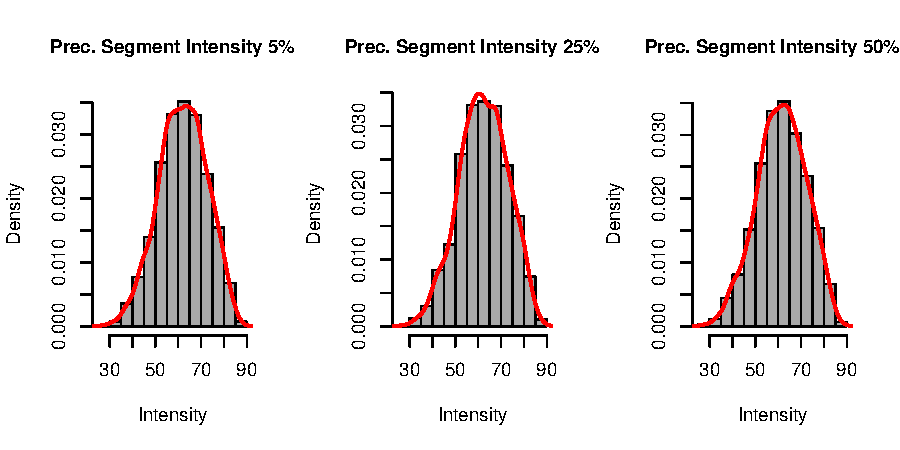
\includegraphics{prelim-019}
  \caption{Density Histograms of Preceding Segment Intensities}
  \label{fig:prec.intensity}
  \end{center}
\end{figure}

\begin{figure}[h!]
  \begin{center}
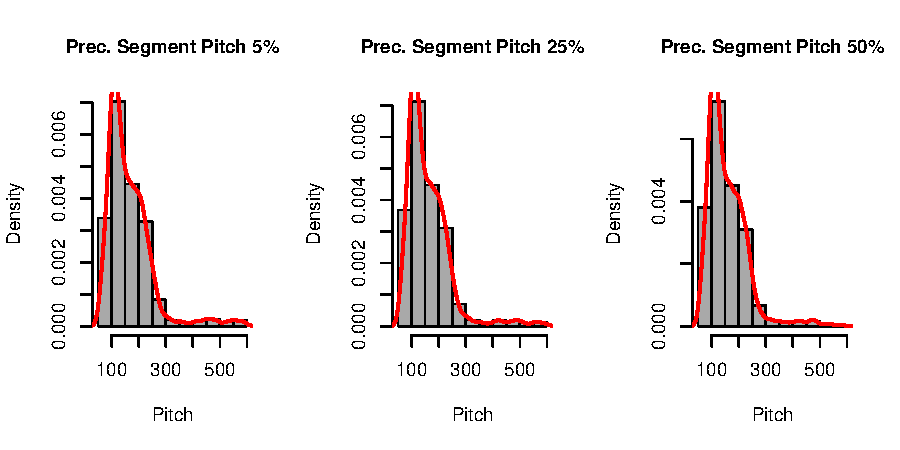
\includegraphics{prelim-021}
  \caption{Density Histograms of Preceding Segment Pitches}
  \label{fig:prec.pitch}
  \end{center}
\end{figure}

\newpage
\subsection*{Random Effects}
\addcontentsline{toc}{subsection}{Random Effects}
There are two random effects in this data: speaker and word.  How the
relationship between speaker, word, and token is defined could
potentially make a huge impact on the results and warrants careful
consideration. Out of 3,119 tokens, there are 1,295 unique words among
the sixty-seven speakers; 790 of those occur in just one token\footnote{
  This makes sense.  According to Zipf's Law, the frequencies of words
  in any given corpus are inversely proportional to their rank.  Even
  though this data is a sample of specific types of words from within
  a corpus, it should still follow a power law distribution (at least approximately).\\
  \url{http://en.wikipedia.org/wiki/Zipf\%27s_law}
}.  Speakers used as few as twenty-one and as many as forty-nine
unique words, with a median count of forty (see Appendix \ref{a:res}).

The simpler model is to consider word and speaker as separate
(crossed) effects.  Word-to-word variability and
speaker-to-speaker variablity are considered separately, and like
words are grouped together regardless of the speaker.  If the speaker
has no bearing on the word this model will fit well.

The other approach would be to nest words inside of speaker.  Here,
words are only grouped together if they are spoken by the same
individual. This
model would consider the variability among the 2,617 unique
word:speaker combinations instead of the 1,295 unique words.  This
model is the best choice if certain speakers prefer certain words (or
types of words).

Conceptually, either structure makes sense, and, given the large number
of unique words relative to both the number of speakers and the number
of tokens, there is not a clearly defined better choice.  To determine
the nature of the relationship, it will come down to modeling the
responses both ways and comparing the results.  If one method consistently
outperforms the other, that will point to the true underlying
structure of the data.



\section*{Dependent Variables}
\addcontentsline{toc}{section}{Dependent Variables}
The responses are all phonetic variables and, taken as a whole, paint
the picture of the sounds that were recorded in the token,
particularly the sibilant and its preceding segment.
The model used for each response is determined
by its distributionality.  Responses that follow Normal Distributions
(or can be easily transformed to) can be modeled with Linear Mixed
Models (LMMs), while responses that follow other well-defined
distributions (such as Binomial or Gamma Distributions) can be modeled
using Generalized Linear Mixed Models (GLMMs).  If any response does
not follow a well-behaved distribution an appropriate non-parametric
model can be used.

\subsection*{Sibilant Duration}
\addcontentsline{toc}{subsection}{Sibilant Duration}
Sibilant Duration is the time, in seconds, it took the speaker to
create that particular sibilant sound.
\begin{figure}[h!]
  \begin{center}
    \begin{minipage}[t]{0.5\linewidth}
      \begin{center}
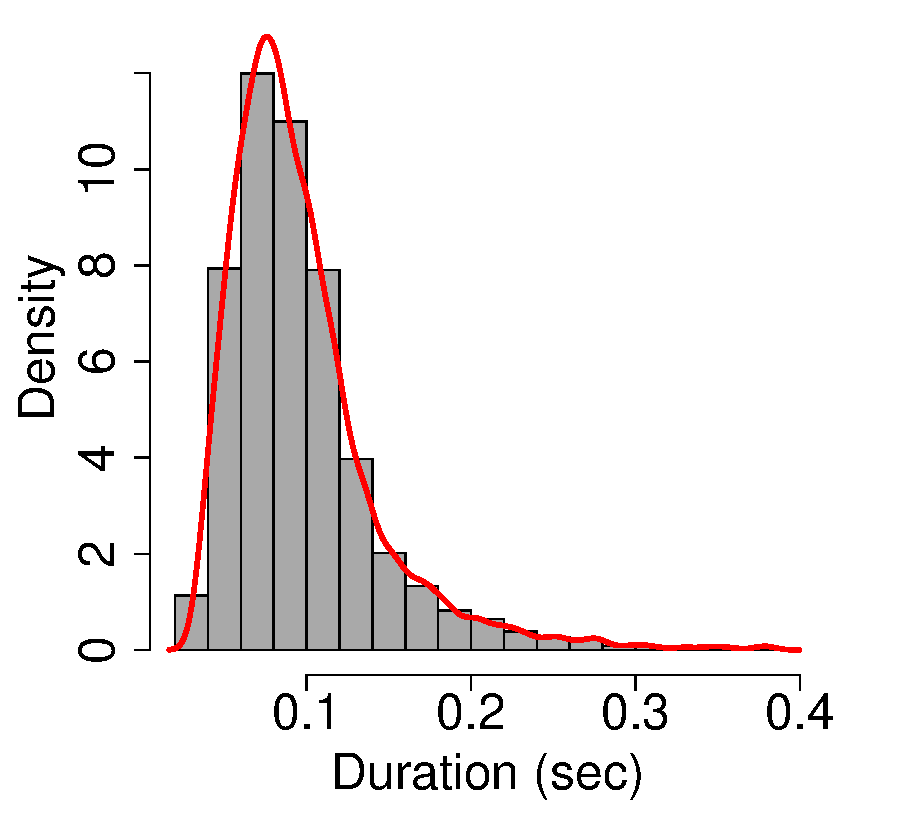
\includegraphics{prelim-026}
      \end{center}
    \end{minipage}
    \caption{Density Histogram of Sibilant Duration}
    \label{fig:sib_dur_hist}
  \end{center}
\end{figure}

The distribution is strictly positive and has significant
right-skew, which is not unexpected.  Time measurements, by nature,
have a lower bound of zero, and, given the relatively short amount of
time it takes to produce a consonant sound, it is not surprising that
the density is highest closer to zero and tapers off as duration increases.

This shape resembles either a Lognormal Distribution (i.e., the
logarithm of the variable has a Normal Distribution) or a Gamma
Distribution.  How closely it follows these distributions can be
evaluated using Quantile--Quantile Plots (Figure \ref{fig:sib_dur_qq}).
In these plots, the points
following an approximately straight line indicate that the
distribution of the variable closely follows the named distribution.

\begin{figure}[h!]
  \begin{center}
    \begin{minipage}[t]{\linewidth}
      \begin{center}
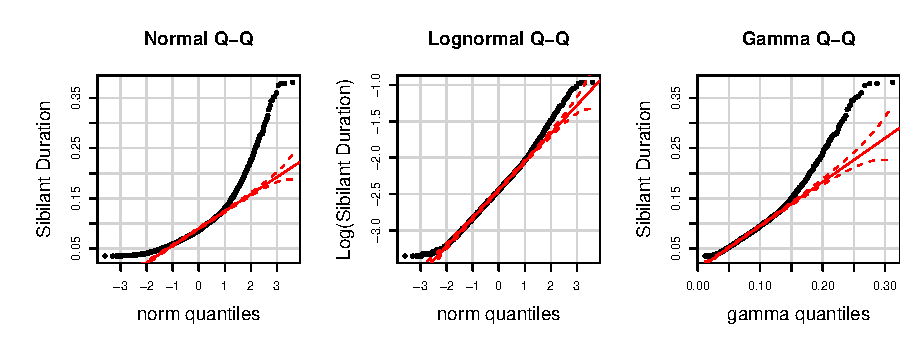
\includegraphics{prelim-028}
      \end{center}
    \end{minipage}
    \caption{Sibilant Duration Quantile--Quantile Plots}
    \label{fig:sib_dur_qq}
  \end{center}
\end{figure}
Since Sibilant Duration most closely follows a Lognormal Distribution,
an LMM will be fit using the logarithm of Sibilant Duration as the response.

\subsection*{Preceding Segment Duration}
\addcontentsline{toc}{subsection}{Preceding Segment Duration}
Similar to Sibilant Duration, Preceding Segment Duration is a
measurement of the time it took to produce the sound preceding the sibilant.

\begin{figure}[h!]
  \begin{center}
    \begin{minipage}[t]{0.5\linewidth}
      \begin{center}
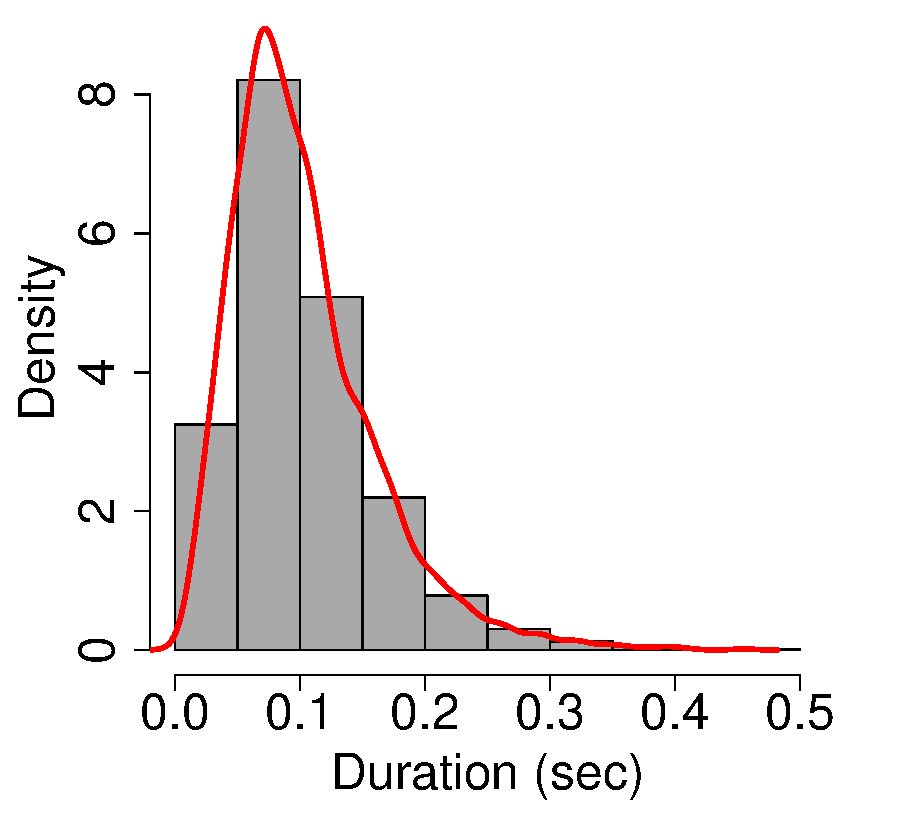
\includegraphics{prelim-030}
      \end{center}
    \end{minipage}
    \caption{Density Histogram of Preceding Segment Duration}
    \label{fig:prec_dur_hist}
  \end{center}
\end{figure}
Again, the distribution is strictly positive and right-skewed.  The
increased variability in Preceding Segment Duration compared to
Sibilant Duration likely comes from the fact that the preceding
segments can be a variety of consonants and vowels, whereas the
sibilant is restricted to only alveolar fricatives.  The same process
of examining Quantile--Quantile Plots is used to select an appropriate
model for Preceding Segment Duration.

\begin{figure}[h!]
  \begin{center}
    \begin{minipage}[t]{\linewidth}
      \begin{center}
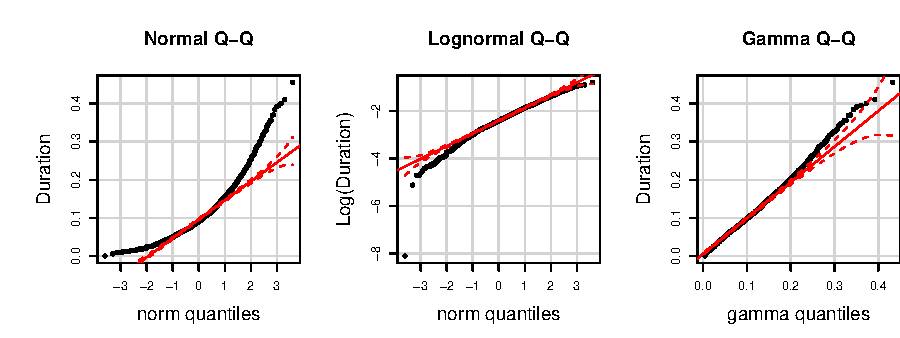
\includegraphics{prelim-032}
      \end{center}
    \end{minipage}
    \caption{Preceding Segment Duration Quantile--Quantile Plots}
    \label{fig:prec_dur_qq}
  \end{center}
\end{figure}

For Preceding Segment Duration, a Gamma GLMM is the best fit.

\subsection*{Center of Gravity}
\addcontentsline{toc}{subsection}{Center of Gravity}
The Center of Gravity (CoG) is the average frequency over the sibilant's
sound spectrum.  Since the tokens were recorded in interviews, two methods
were used to ``clean up the signal'' and filter out any interference
that may distort the Center of Gravity.  One method is to only
consider the middle sixty percent of the signal, which makes sure only
the sibilant itself is being considered and no noise from the preceding
or following segments is bleeding over into the sibilant spectrum.  In
addition to this, the token spectrums were filtered using the Hann
Function, which is a bell-shaped window function, to help eliminate
extraneous noise.

Center of Gravity, then, exists in four different versions: the Full (raw)
CoG, the Middle 60\% CoG, the Filtered CoG, and the Filtered Middle
60\% CoG.  Obviously, these four variables will be highly collinear.
To avoid any of the issues that arise from multicollinearity, it makes
the most sense to only select the version with the smoothest curve, which
is the Filtered Middle 60\% CoG (Figure \ref{fig:cog_hist}).

\begin{figure}[h!]
  \begin{center}
    \begin{minipage}[t]{.9\linewidth}
      \begin{center}
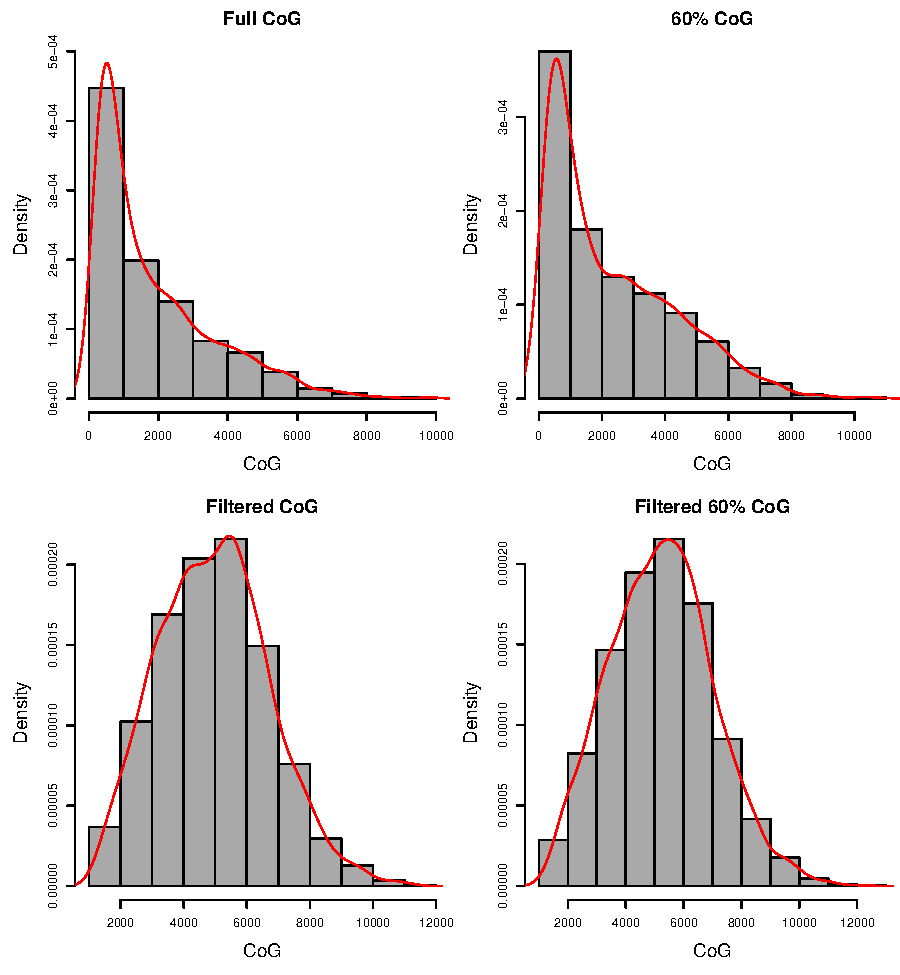
\includegraphics{prelim-034}
      \end{center}
    \end{minipage}
    \caption{Density Histograms of Centers of Gravity}
    \label{fig:cog_hist}
  \end{center}
\end{figure}

\begin{figure}[h!]
  \begin{center}
    \begin{minipage}[t]{.4\linewidth}
      \begin{center}
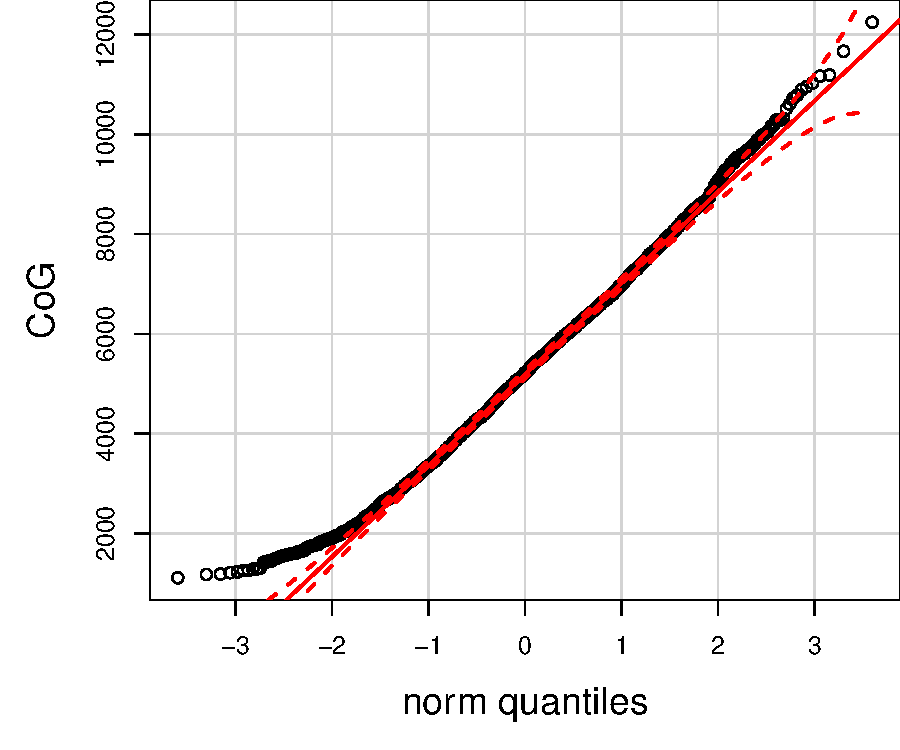
\includegraphics{prelim-036}
      \end{center}
    \end{minipage}
    \caption{Normal Quantile--Quantile Plot for Filtered 60\% CoG}
    \label{fig:cog_qq}
  \end{center}
\end{figure}
\newpage
While  the distribution isn't perfectly Normal (Figure
\ref{fig:cog_qq}), a straightforward LMM should be sufficient for
modeling the Center of Gravity.


\newpage
\subsection*{Percent Voicelessness}
\addcontentsline{toc}{subsection}{Percent Voicelessness}
Percent Voicelessness as a variable name is slightly misleading.  This
variable is a measure of the percent of the sibilant's duration that
lacks glottal pulsing, and, as discussed previously, this is only one
part of what determines whether a sound is voiced or voiceless.  As
Figure \ref{fig:vls_hist} shows, Percent Voicelessness is continuous,
bimodal, and bounded by zero and one.   As such, it most likely follows a Beta
Distribution with shape parameters less than one.

\begin{figure}[h!]
  \begin{center}
    \begin{minipage}[t]{0.6\linewidth}
      \begin{center}
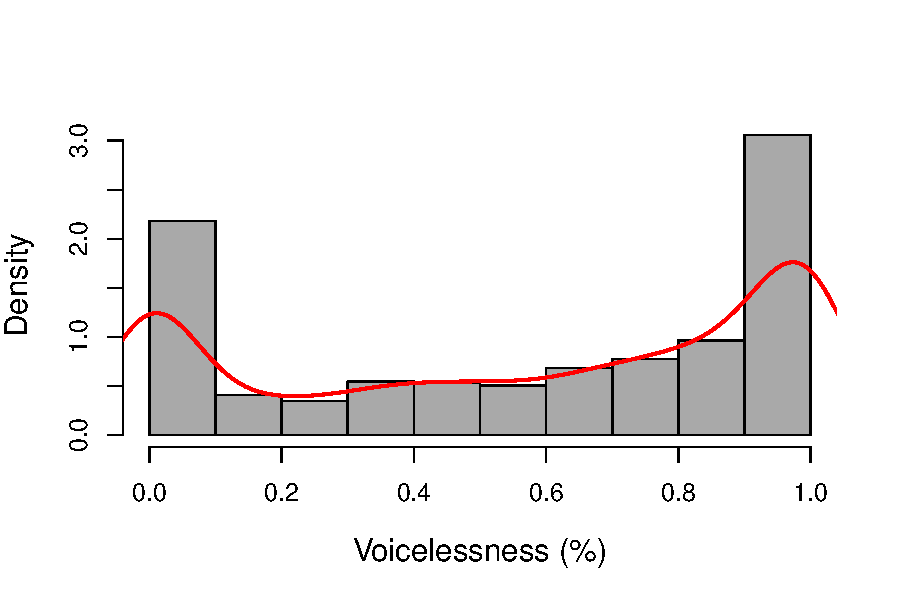
\includegraphics{prelim-038}
      \end{center}
    \end{minipage}
    \caption{Density Histogram of Percent Voicelessness}
    \label{fig:vls_hist}
  \end{center}
\end{figure}

\begin{figure}[h!]
  \begin{center}
    \begin{minipage}[t]{0.6\linewidth}
      \begin{center}
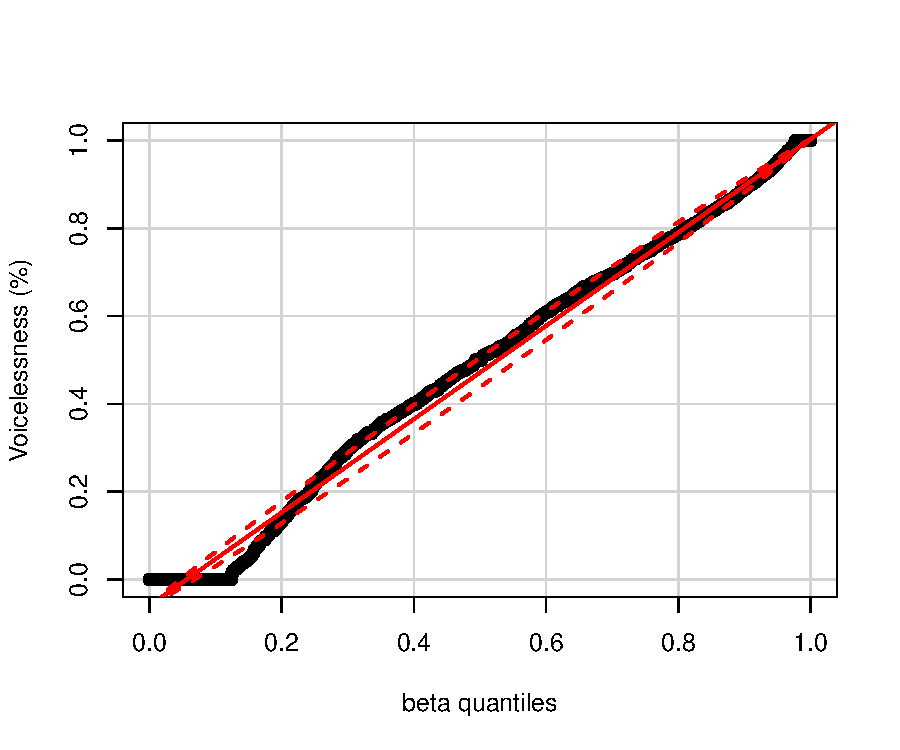
\includegraphics{prelim-040}
      \end{center}
    \end{minipage}
    \caption{Beta Quantile--Quantile Plot of Percent Voicelessness\\
      ($\alpha=0.5, \beta=0.35$)}
    \label{fig:vls_qq}
  \end{center}
\end{figure}

Beta Distributions, by their restricted nature,  present unique
challenges for modeling.  This could possibily be modeled as a GLMM
with a logit link function, but it may be best to use Beta Regression\footnote{
  \url{http://cran.r-project.org/web/packages/betareg/vignettes/betareg-ext.pdf}
} or some kind of non-parametric regression.  This will be explored later.

\newpage
\section*{Analysis}
\addcontentsline{toc}{section}{Analysis}
For each response there are seven social variables, fourteen linguistic
variables, and three covariates, for a total of twenty-four predictors
that need to be evaluated. Even if models are restricted to only those
with two-factor interactions, that adds another 276 potential terms.
Given this complex nature, backward variable selection
techniques will be avoided in favor of forward
selection.  As this analysis is continued, the approach to variable
selection will be refined.

Unfortunately, the functionality is not yet included in any R package
to automatically apply forward selection techniques to mixed effects
models.  Rense Nieuwenhuis, a sociologist from Swedish Institute for
Social Research (SOFI) of Stockholm University,
publicly released his code for a function that implements a basic
stepwise function for forward selection with mixed effects models.  It
works by iteratively fitting models with added terms and comparing
them using a (ML) likelihood ratio test\footnotemark.

\footnotetext{
  As this is an unpublished package that has never been formally
  peer-reviewed, its methodology and results need to be verified
  before we run with them.\\
  \url{http://www.rensenieuwenhuis.nl/r-sessions-32/}
}


Hox outlines a step-up procedure for variable selection in
mixed effects models which will be (mostly) followed here\footnotemark.
\begin{enumerate}
  \item Fit a model with only the random intercepts.  Instead of an
    intercept only model, selection will start with the other
    responses as covariates.
  \item Determine significant fixed effects at the observation level
    (low level effects).
  \item Determine significant fixed effects at the group level.  In
    this study, these are the social variables (which describe the
    speaker) and the morphological/phonological variables (which
    describe the word).
  \item Explore the random effects structure.
\end{enumerate}

\footnotetext{
  Hox, J. J. (2002). Multilevel analysis techniques and
  applications. Mahwah, N.J.: Lawrence Erlbaum Associates. (45-50).
}



In addition to using a log transformation for Sibilant Duration,
several variables should be scaled.  Center of Gravity ranges from
1,112--12,250 Hz,  durations range from 0.035--0.445
sec., the intensities range from 23.11--89.47 dB, and Percent
Voicelessness is in the unit interval (0--1).  Scaling CoG, the pitches, and the
intensities will lead to coefficients that are easier to compare (with
the added benefit of reducing collinearity).

For the time being interactions will only be considered between variables of the same
type (e.g., interactions among social variables
and among morphological variables, but not between them) and a few
other interactions of interest (such as sibilant location and standard
pronunciation).  Also worth noting is that model comparisons are only
meaningful if the models are based on the same data.  Because of this,
any row that contains a missing value will have to be omitted.


\subsection*{Sibilant Duration}
\addcontentsline{toc}{subsection}{Sibilant Duration}
\subsubsection*{Base Model}

\begingroup
        \catcode`_=\active
        \gdef\works{
           \catcode`_=\active
           \def_{\textunderscore\-}%
        }\texttt{Linear mixed model fit by REML \newline Formula:\newline lme4::lmer(formula = log(sib_dur) ~ prec_segment_dur + sib.cog +
    vls_percent + (1 | word) + (1 | speaker), data = dat2)
\newline\newline REML at convergence:  1717.105 \newline \newline Random Effects:\newline % latex table generated in R 3.1.1 by xtable 1.7-3 package
% Fri Aug  8 14:30:19 2014
\begin{tabular}{llrr}
  \hline
Groups & Name & Variance & St.Dev. \\
  \hline
word & (Intercept) & 0.01 & 0.11 \\
  speaker & (Intercept) & 0.02 & 0.15 \\
  Residual &  & 0.10 & 0.32 \\
   \hline
\end{tabular}
\newline Number of obs: 2437, groups: word, 1074; speaker, 67\newline \newline Fixed Effects:\newline % latex table generated in R 3.1.1 by xtable 1.7-3 package
% Fri Aug  8 14:30:19 2014
\begin{tabular}{rrrrrr}
  \hline
 & Estimate & Std. Error & df & t value & Pr($>$$|$t$|$) \\
  \hline
(Intercept) & -2.812 & 0.026 & 197.529 & -107.354 & 0.000 \\
  prec\_segment\_dur & 1.836 & 0.129 & 1915.706 & 14.180 & 0.000 \\
  sib.cog & 0.096 & 0.010 & 1386.651 & 9.432 & 0.000 \\
  vls\_percent & 0.318 & 0.021 & 2398.252 & 14.965 & 0.000 \\
   \hline
\end{tabular}
}\endgroup\newline
\subsubsection*{Selecting Low Level Fixed Effects}
Now the low level effects (those collected at the token level) can
be added to the model using forward selection.\newline

\begingroup
        \catcode`_=\active
        \gdef\works{
           \catcode`_=\active
           \def_{\textunderscore\-}%
        }\texttt{Linear mixed model fit by REML \newline Formula:\newline lme4::lmer(formula = log(sib_dur) ~ prec_segment_dur + sib.cog +
    vls_percent + (1 | word) + (1 | speaker) + prec.int25 + prec.pitch50 +
    prec.pitch05:prec.pitch50, data = dat2)
\newline\newline REML at convergence:  1722.39 \newline \newline Random Effects:\newline % latex table generated in R 3.1.1 by xtable 1.7-3 package
% Fri Aug  8 14:30:22 2014
\begin{tabular}{llrr}
  \hline
Groups & Name & Variance & St.Dev. \\
  \hline
word & (Intercept) & 0.01 & 0.11 \\
  speaker & (Intercept) & 0.02 & 0.15 \\
  Residual &  & 0.10 & 0.32 \\
   \hline
\end{tabular}
\newline Number of obs: 2437, groups: word, 1074; speaker, 67\newline \newline Fixed Effects:\newline % latex table generated in R 3.1.1 by xtable 1.7-3 package
% Fri Aug  8 14:30:22 2014
\begin{tabular}{rrrrrr}
  \hline
 & Estimate & Std. Error & df & t value & Pr($>$$|$t$|$) \\
  \hline
(Intercept) & -2.819 & 0.026 & 194.067 & -106.875 & 0.000 \\
  prec\_segment\_dur & 1.927 & 0.131 & 1974.257 & 14.681 & 0.000 \\
  sib.cog & 0.097 & 0.010 & 1540.440 & 9.477 & 0.000 \\
  vls\_percent & 0.304 & 0.021 & 2385.997 & 14.185 & 0.000 \\
  prec.int25 & -0.033 & 0.013 & 625.374 & -2.641 & 0.008 \\
  prec.pitch50 & -0.025 & 0.012 & 1741.743 & -2.192 & 0.029 \\
  prec.pitch50:prec.pitch05 & 0.013 & 0.004 & 2209.404 & 2.952 & 0.003 \\
   \hline
\end{tabular}
}\endgroup\newline\newline\newline\texttt{Selection completed in 6.8 minutes.}\newline\newline
This model has an interaction that includes \texttt{prec.pitch05}, which
was not left in the model on its own.

\begin{Schunk}
\begin{Sinput}
> sib.dur.1.1 <- update(sib.dur.1, . ~ . + prec.pitch05)
\end{Sinput}
\end{Schunk}
% latex table generated in R 3.1.1 by xtable 1.7-3 package
% Fri Aug  8 14:30:22 2014
\begin{table}[h!]
\centering
\begin{tabular}{lrrrrrrrr}
  \hline
 & Df & AIC & BIC & logLik & deviance & Chisq & Chi Df & Pr($>$Chisq) \\
  \hline
sib.dur.1 & 10 & 1696.94 & 1754.92 & -838.47 & 1676.94 &  &  &  \\
  sib.dur.1.1 & 11 & 1698.83 & 1762.61 & -838.41 & 1676.83 & 0.11 & 1 & 0.7442 \\
   \hline
\end{tabular}
\end{table}
While there is no real difference in the fit of the models,
first-order terms always need to be included if their interactions are.\newline

\begingroup
        \catcode`_=\active
        \gdef\works{
           \catcode`_=\active
           \def_{\textunderscore\-}%
        }\texttt{Linear mixed model fit by REML \newline Formula:\newline lme4::lmer(formula = log(sib_dur) ~ prec_segment_dur + sib.cog +
    vls_percent + (1 | word) + (1 | speaker) + prec.int25 + prec.pitch50 +
    prec.pitch05 + prec.pitch50:prec.pitch05, data = dat2)
\newline\newline REML at convergence:  1729.261 \newline \newline Random Effects:\newline % latex table generated in R 3.1.1 by xtable 1.7-3 package
% Fri Aug  8 14:30:23 2014
\begin{tabular}{llrr}
  \hline
Groups & Name & Variance & St.Dev. \\
  \hline
word & (Intercept) & 0.01 & 0.11 \\
  speaker & (Intercept) & 0.02 & 0.14 \\
  Residual &  & 0.10 & 0.32 \\
   \hline
\end{tabular}
\newline Number of obs: 2437, groups: word, 1074; speaker, 67\newline \newline Fixed Effects:\newline % latex table generated in R 3.1.1 by xtable 1.7-3 package
% Fri Aug  8 14:30:23 2014
\begin{tabular}{rrrrrr}
  \hline
 & Estimate & Std. Error & df & t value & Pr($>$$|$t$|$) \\
  \hline
(Intercept) & -2.819 & 0.026 & 195.420 & -106.757 & 0.000 \\
  prec\_segment\_dur & 1.928 & 0.131 & 1971.419 & 14.681 & 0.000 \\
  sib.cog & 0.097 & 0.010 & 1538.381 & 9.474 & 0.000 \\
  vls\_percent & 0.305 & 0.021 & 2384.629 & 14.187 & 0.000 \\
  prec.int25 & -0.033 & 0.013 & 618.644 & -2.615 & 0.009 \\
  prec.pitch50 & -0.023 & 0.014 & 2267.101 & -1.617 & 0.106 \\
  prec.pitch05 & -0.004 & 0.012 & 2356.820 & -0.323 & 0.747 \\
  prec.pitch50:prec.pitch05 & 0.013 & 0.004 & 2194.657 & 2.969 & 0.003 \\
   \hline
\end{tabular}
}\endgroup\newline
\subsubsection*{Selecting High Level Fixed Effects}
Fixed effects collected at the group level can now be considered.\newline

\begingroup
        \catcode`_=\active
        \gdef\works{
           \catcode`_=\active
           \def_{\textunderscore\-}%
        }\texttt{Linear mixed model fit by REML \newline Formula:\newline lme4::lmer(formula = log(sib_dur) ~ prec_segment_dur + sib.cog +
    vls_percent + (1 | word) + (1 | speaker) + prec.int25 + prec.pitch50 +
    prec.pitch05 + age_group + prec.pitch50:prec.pitch05 + sib.combined:following.type,
    data = dat2)
\newline\newline REML at convergence:  1303.739 \newline \newline Random Effects:\newline % latex table generated in R 3.1.1 by xtable 1.7-3 package
% Fri Aug  8 14:30:26 2014
\begin{tabular}{llrr}
  \hline
Groups & Name & Variance & St.Dev. \\
  \hline
word & (Intercept) & 0.00 & 0.06 \\
  speaker & (Intercept) & 0.01 & 0.12 \\
  Residual &  & 0.09 & 0.30 \\
   \hline
\end{tabular}
\newline Number of obs: 2437, groups: word, 1074; speaker, 67\newline \newline Fixed Effects:\newline % latex table generated in R 3.1.1 by xtable 1.7-3 package
% Fri Aug  8 14:30:26 2014
\begin{tabular}{rrrrrr}
  \hline
 & Estimate & Std. Error & df & t value & Pr($>$$|$t$|$) \\
  \hline
(Intercept) & -2.758 & 0.033 & 135.396 & -82.922 & 0.000 \\
  prec\_segment\_dur & 1.436 & 0.120 & 1370.917 & 11.938 & 0.000 \\
  sib.cog & 0.085 & 0.009 & 1393.879 & 9.122 & 0.000 \\
  vls\_percent & 0.191 & 0.021 & 2345.222 & 9.078 & 0.000 \\
  prec.int25 & -0.017 & 0.011 & 499.649 & -1.476 & 0.141 \\
  prec.pitch50 & -0.015 & 0.013 & 2261.748 & -1.192 & 0.233 \\
  prec.pitch05 & -0.000 & 0.011 & 2392.557 & -0.045 & 0.964 \\
  age\_groupgroup\_3 & -0.126 & 0.038 & 60.488 & -3.303 & 0.002 \\
  age\_groupgroup\_4 & -0.144 & 0.039 & 59.642 & -3.695 & 0.000 \\
  prec.pitch50:prec.pitch05 & 0.007 & 0.004 & 2191.216 & 1.791 & 0.073 \\
  sib.combined[s]:following.typecons. & 0.190 & 0.024 & 807.619 & 7.876 & 0.000 \\
  sib.combined[z]:following.typecons. & 0.014 & 0.018 & 1485.596 & 0.741 & 0.459 \\
  sib.combined[s]:following.typepause & 0.510 & 0.035 & 1553.364 & 14.595 & 0.000 \\
  sib.combined[z]:following.typepause & 0.418 & 0.025 & 2067.947 & 17.007 & 0.000 \\
  sib.combined[s]:following.typevowel & 0.213 & 0.021 & 878.092 & 10.320 & 0.000 \\
   \hline
\end{tabular}
}\endgroup\newline\newline\newline\texttt{Selection completed in 7.47 minutes.}\newline\newline
By adding in the high level effects, the word-to-word
variability has been reduced substantially, and the speaker-to-speaker
and token-to-token variability marginally.  At the same time,
\texttt{prec.int25} is no longer significant, and its removal can be
evaluated.  Like with the low level variable selection, there are
interactions included in this model that are missing first-order terms
(\texttt{following.type} and \texttt{sib.combined}), and  this needs
to be corrected first.

\begin{Schunk}
\begin{Sinput}
> sib.dur.2.0 <- update(sib.dur.2, .~. + following.type + sib.combined)
\end{Sinput}
\end{Schunk}
\begingroup
        \catcode`_=\active
        \gdef\works{
           \catcode`_=\active
           \def_{\textunderscore\-}%
        }\texttt{Linear mixed model fit by REML \newline Formula:\newline lme4::lmer(formula = log(sib_dur) ~ prec_segment_dur + sib.cog +
    vls_percent + (1 | word) + (1 | speaker) + prec.int25 + prec.pitch50 +
    prec.pitch05 + age_group + following.type + sib.combined +
    prec.pitch50:prec.pitch05 + sib.combined:following.type,
    data = dat2)
\newline\newline REML at convergence:  1303.739 \newline \newline Random Effects:\newline % latex table generated in R 3.1.1 by xtable 1.7-3 package
% Fri Aug  8 14:30:28 2014
\begin{tabular}{llrr}
  \hline
Groups & Name & Variance & St.Dev. \\
  \hline
word & (Intercept) & 0.00 & 0.06 \\
  speaker & (Intercept) & 0.01 & 0.12 \\
  Residual &  & 0.09 & 0.30 \\
   \hline
\end{tabular}
\newline Number of obs: 2437, groups: word, 1074; speaker, 67\newline \newline Fixed Effects:\newline % latex table generated in R 3.1.1 by xtable 1.7-3 package
% Fri Aug  8 14:30:28 2014
\begin{tabular}{rrrrrr}
  \hline
 & Estimate & Std. Error & df & t value & Pr($>$$|$t$|$) \\
  \hline
(Intercept) & -2.568 & 0.037 & 197.418 & -69.655 & 0.000 \\
  prec\_segment\_dur & 1.436 & 0.120 & 1370.918 & 11.938 & 0.000 \\
  sib.cog & 0.085 & 0.009 & 1393.879 & 9.122 & 0.000 \\
  vls\_percent & 0.191 & 0.021 & 2345.222 & 9.078 & 0.000 \\
  prec.int25 & -0.017 & 0.011 & 499.649 & -1.476 & 0.141 \\
  prec.pitch50 & -0.015 & 0.013 & 2261.748 & -1.192 & 0.233 \\
  prec.pitch05 & -0.000 & 0.011 & 2392.557 & -0.045 & 0.964 \\
  age\_groupgroup\_3 & -0.126 & 0.038 & 60.488 & -3.303 & 0.002 \\
  age\_groupgroup\_4 & -0.144 & 0.039 & 59.642 & -3.695 & 0.000 \\
  following.typepause & 0.320 & 0.035 & 2359.026 & 9.023 & 0.000 \\
  following.typevowel & 0.023 & 0.023 & 1631.346 & 1.034 & 0.301 \\
  sib.combined[z] & -0.176 & 0.023 & 882.451 & -7.569 & 0.000 \\
  prec.pitch50:prec.pitch05 & 0.007 & 0.004 & 2191.216 & 1.791 & 0.073 \\
  following.typepause:sib.combined[z] & 0.084 & 0.042 & 2381.074 & 1.992 & 0.046 \\
  following.typevowel:sib.combined[z] & -0.037 & 0.029 & 1629.832 & -1.272 & 0.203 \\
   \hline
\end{tabular}
}\endgroup\newline\newline\newline
Interestingly, despite these terms not being selected by the step
function, they are highly significant.

\begin{Schunk}
\begin{Sinput}
> sib.dur.2.1 <- update(sib.dur.2.0, . ~ . - prec.int25)
\end{Sinput}
\end{Schunk}

% latex table generated in R 3.1.1 by xtable 1.7-3 package
% Fri Aug  8 14:30:29 2014
\begin{table}[ht]
\centering
\begin{tabular}{lrrrrrrrr}
  \hline
 & Df & AIC & BIC & logLik & deviance & Chisq & Chi Df & Pr($>$Chisq) \\
  \hline
sib.dur.2.1 & 17 & 1246.64 & 1345.22 & -606.32 & 1212.64 &  &  &  \\
  sib.dur.2.0 & 18 & 1246.43 & 1350.81 & -605.22 & 1210.43 & 2.21 & 1 & 0.1372 \\
   \hline
\end{tabular}
\end{table}
Having \texttt{prec.int25} is no better than not having it in the model, so
it is safe to drop the term.\newline

\begingroup
        \catcode`_=\active
        \gdef\works{
           \catcode`_=\active
           \def_{\textunderscore\-}%
        }\texttt{Linear mixed model fit by REML \newline Formula:\newline lme4::lmer(formula = log(sib_dur) ~ prec_segment_dur + sib.cog +
    vls_percent + (1 | word) + (1 | speaker) + prec.pitch50 +
    prec.pitch05 + age_group + following.type + sib.combined +
    prec.pitch50:prec.pitch05 + following.type:sib.combined,
    data = dat2)
\newline\newline REML at convergence:  1298.8 \newline \newline Random Effects:\newline % latex table generated in R 3.1.1 by xtable 1.7-3 package
% Fri Aug  8 14:30:30 2014
\begin{tabular}{llrr}
  \hline
Groups & Name & Variance & St.Dev. \\
  \hline
word & (Intercept) & 0.00 & 0.06 \\
  speaker & (Intercept) & 0.01 & 0.12 \\
  Residual &  & 0.09 & 0.30 \\
   \hline
\end{tabular}
\newline Number of obs: 2437, groups: word, 1074; speaker, 67\newline \newline Fixed Effects:\newline % latex table generated in R 3.1.1 by xtable 1.7-3 package
% Fri Aug  8 14:30:30 2014
\begin{tabular}{rrrrrr}
  \hline
 & Estimate & Std. Error & df & t value & Pr($>$$|$t$|$) \\
  \hline
(Intercept) & -2.573 & 0.037 & 199.384 & -70.042 & 0.000 \\
  prec\_segment\_dur & 1.400 & 0.118 & 1285.856 & 11.881 & 0.000 \\
  sib.cog & 0.086 & 0.009 & 1311.384 & 9.307 & 0.000 \\
  vls\_percent & 0.196 & 0.021 & 2364.551 & 9.422 & 0.000 \\
  prec.pitch50 & -0.017 & 0.013 & 2346.514 & -1.345 & 0.179 \\
  prec.pitch05 & -0.001 & 0.011 & 2390.419 & -0.122 & 0.903 \\
  age\_groupgroup\_3 & -0.126 & 0.038 & 61.411 & -3.306 & 0.002 \\
  age\_groupgroup\_4 & -0.140 & 0.039 & 60.411 & -3.613 & 0.001 \\
  following.typepause & 0.325 & 0.035 & 2354.153 & 9.183 & 0.000 \\
  following.typevowel & 0.023 & 0.023 & 1622.177 & 1.028 & 0.304 \\
  sib.combined[z] & -0.173 & 0.023 & 850.412 & -7.473 & 0.000 \\
  prec.pitch50:prec.pitch05 & 0.008 & 0.004 & 2310.532 & 1.991 & 0.047 \\
  following.typepause:sib.combined[z] & 0.083 & 0.042 & 2383.381 & 1.961 & 0.050 \\
  following.typevowel:sib.combined[z] & -0.037 & 0.029 & 1621.454 & -1.265 & 0.206 \\
   \hline
\end{tabular}
}\endgroup\newline
\subsubsection*{Comparing Grouping Structures}
Now that the fixed effects that most contribute to the optimal model
have been identified, the best random effects structure can be
explored.  Up to now, the usual interpretation of word crossed with
speaker has been used.  If, for example, there are speakers who tend
to use more [s]'s than [z]'s, a nested structure
where unique word:speaker combinations are considered instead of unique
words may be better.\newline

\begingroup
        \catcode`_=\active
        \gdef\works{
           \catcode`_=\active
           \def_{\textunderscore\-}%
        }\texttt{Linear mixed model fit by REML \newline Formula:\newline lme4::lmer(formula = log(sib_dur) ~ prec_segment_dur + sib.cog +
    vls_percent + prec.pitch50 + prec.pitch05 + age_group + following.type +
    sib.combined + (1 | speaker/word) + \newline prec.pitch50:prec.pitch05 +
    following.type:sib.combined, data = dat2)
\newline\newline REML at convergence:  1291.545 \newline \newline Random Effects:\newline % latex table generated in R 3.1.1 by xtable 1.7-3 package
% Fri Aug  8 14:30:32 2014
\begin{tabular}{llrr}
  \hline
Groups & Name & Variance & St.Dev. \\
  \hline
word:speaker & (Intercept) & 0.02 & 0.13 \\
  speaker & (Intercept) & 0.01 & 0.12 \\
  Residual &  & 0.08 & 0.28 \\
   \hline
\end{tabular}
\newline Number of obs: 2437, groups: word, 2108; speaker, 67\newline \newline Fixed Effects:\newline % latex table generated in R 3.1.1 by xtable 1.7-3 package
% Fri Aug  8 14:30:32 2014
\begin{tabular}{rrrrrr}
  \hline
 & Estimate & Std. Error & df & t value & Pr($>$$|$t$|$) \\
  \hline
(Intercept) & -2.572 & 0.037 & 187.767 & -70.191 & 0.000 \\
  prec\_segment\_dur & 1.352 & 0.116 & 2306.424 & 11.676 & 0.000 \\
  sib.cog & 0.089 & 0.009 & 1360.144 & 9.593 & 0.000 \\
  vls\_percent & 0.197 & 0.021 & 2371.304 & 9.495 & 0.000 \\
  prec.pitch50 & -0.016 & 0.013 & 2350.853 & -1.252 & 0.211 \\
  prec.pitch05 & -0.002 & 0.011 & 2390.327 & -0.216 & 0.829 \\
  age\_groupgroup\_3 & -0.126 & 0.039 & 61.662 & -3.271 & 0.002 \\
  age\_groupgroup\_4 & -0.141 & 0.039 & 60.710 & -3.588 & 0.001 \\
  following.typepause & 0.328 & 0.035 & 2301.399 & 9.329 & 0.000 \\
  following.typevowel & 0.023 & 0.022 & 2376.263 & 1.045 & 0.296 \\
  sib.combined[z] & -0.174 & 0.022 & 2352.309 & -7.779 & 0.000 \\
  prec.pitch50:prec.pitch05 & 0.007 & 0.004 & 2335.284 & 1.883 & 0.060 \\
  following.typepause:sib.combined[z] & 0.081 & 0.042 & 2356.043 & 1.936 & 0.053 \\
  following.typevowel:sib.combined[z] & -0.036 & 0.029 & 2373.186 & -1.249 & 0.212 \\
   \hline
\end{tabular}
}\endgroup\newline\newline\newline
The significance of the coefficients did not change very much, but
the nested model has more word-to-word variability and less residual
token-to-token variability when compared to the crossed model.

% latex table generated in R 3.1.1 by xtable 1.7-3 package
% Fri Aug  8 14:30:33 2014
\begin{table}[ht]
\centering
\begin{tabular}{lrrrrrrrr}
  \hline
 & Df & AIC & BIC & logLik & deviance & Chisq & Chi Df & Pr($>$Chisq) \\
  \hline
Crossed & 17 & 1246.64 & 1345.22 & -606.32 & 1212.64 &  &  &  \\
  Nested & 17 & 1239.18 & 1337.76 & -602.59 & 1205.18 & 7.46 & 0 & 0.0000 \\
   \hline
\end{tabular}
\end{table}
The fit of the model with the nested structure is significantly better
than the fit of the model with the crossed structure.

\subsubsection*{Model Diagnostics}
To verify that this model is appropriate, we need to check that the residuals
are independent of each other and Normally distributed with a mean of
zero (residuals being the difference between the predicted response
and the actual response for every token).

The assumption of Normality can be verified with a Quantile--Quantile
Plot and independence and mean by plotting the
residuals against their index (Figure \ref{fig:sib.dur.res}).  The
residuals should form a straight line in the Normal Q--Q Plot, and
they should be randomly scattered about zero (on the y-axis) in the Residual by Index Plot.


\begin{figure}[h!]
  \begin{center}
    \begin{minipage}[t]{0.8\linewidth}
      \begin{center}
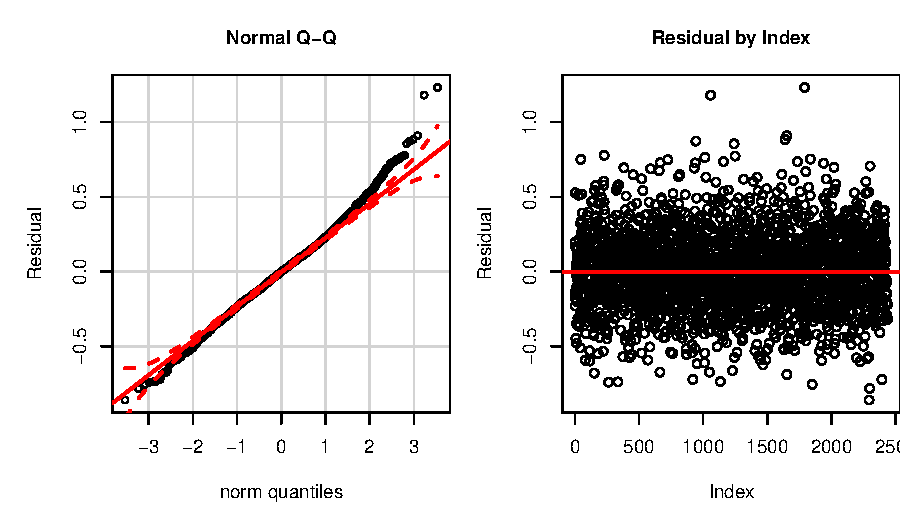
\includegraphics{prelim-056}
      \end{center}
    \end{minipage}
    \caption{Diagnostic Plots}
    \label{fig:sib.dur.res}
  \end{center}
\end{figure}

The slight curvature at the top of the Q--Q Plot, along with the
slightly higher number of positive residuals at the top of the
Residual by Index Plot show that there may be a slight right-skew in
the residuals, but this is not enough to be troubling.

\subsubsection*{Interpretation}
This first caveat with interpreting this model is dealing with
transformations that were used.  Several variables were centered and
scaled (standardized), and the response was the natural logarithm of
Sibilant Duration, not Sibilant Duration itself.  These
transformations would be a complication if the model was intended for
prediction. Fortunately, this study  only concerned with identifying
relationships between these variables, and neither scaling the
predictors nor log-transforming the response affect these
interpretations.

An increase or decrease in the logarithm of Sibilant Duration would also be an
change of the same direction in Sibilant Duration, and the same holds true for scaling the
independent variables.  A simple interpretation of
variable coefficients for log-transformed responses is that  a
one-unit change in the independent variable (with all others held
constant) will result in a change in the dependent variable of
$100\cdot($coefficient$)$\%.  Positive coefficients represent an
increase in the response, and negative coefficients represent a decrease\footnote{
  More accurately, for a coefficient $\hat{\beta}$, a one-unit change in the
  independent variable $x$ multiplies the expected value of the response
  by $e^{\hat{\beta}}$.  For small values of $\hat{\beta}$ like we
  have here, the percent change is a useful approximation.
}.

For the scaled variables, a one-unit change is one standard deviation
of that variable.  For the categorical variables, R chooses one level
to be the base value, and the coefficients represent the change in the
response when changing the level.

It is also important to keep in mind with
mixed effects models that the coefficients are the estimated average
effect among all of the groups, so the p-values should not be treated
as gospel.  A coefficient with a p-value of $0.06$ may be important to
the model, and one with a coefficient of $0.04$ may not be all that important
to the practical interpretation.  For now, the decision about whether to focus on
coefficients that are close (on either side) to
$0.05$ will be based on weighing how significant they are against
their effect size.  For example, the interaction
\texttt{prec.pitch50:prec.pitch05} is marginally significant, but
its coefficient is only $0.007$, which represents a change in expected
Sibilant Duration of only $0.7$\%.  This change may or may not be
statistically significant, but, practically, that is not much of a
difference.  The \texttt{following.typepause:sib.combined[z]}
interaction could also go either way, but it represents a change of
$8.1$\% in Sibilant Duration and is probably worth following up on.

% latex table generated in R 3.1.1 by xtable 1.7-3 package
% Fri Aug  8 14:30:34 2014
\begin{table}[h!]
\centering
\begin{tabular}{rrrrrr}
  \hline
 & Estimate & Std. Error & df & t value & Pr($>$$|$t$|$) \\
  \hline
(Intercept) & -2.572 & 0.037 & 187.767 & -70.191 & 0.000 \\
  prec\_segment\_dur & 1.352 & 0.116 & 2306.424 & 11.676 & 0.000 \\
  sib.cog & 0.089 & 0.009 & 1360.144 & 9.593 & 0.000 \\
  vls\_percent & 0.197 & 0.021 & 2371.304 & 9.495 & 0.000 \\
  prec.pitch50 & -0.016 & 0.013 & 2350.853 & -1.252 & 0.211 \\
  prec.pitch05 & -0.002 & 0.011 & 2390.327 & -0.216 & 0.829 \\
  age\_groupgroup\_3 & -0.126 & 0.039 & 61.662 & -3.271 & 0.002 \\
  age\_groupgroup\_4 & -0.141 & 0.039 & 60.710 & -3.588 & 0.001 \\
  following.typepause & 0.328 & 0.035 & 2301.399 & 9.329 & 0.000 \\
  following.typevowel & 0.023 & 0.022 & 2376.263 & 1.045 & 0.296 \\
  sib.combined[z] & -0.174 & 0.022 & 2352.309 & -7.779 & 0.000 \\
  prec.pitch50:prec.pitch05 & 0.007 & 0.004 & 2335.284 & 1.883 & 0.060 \\
  following.typepause:sib.combined[z] & 0.081 & 0.042 & 2356.043 & 1.936 & 0.053 \\
  following.typevowel:sib.combined[z] & -0.036 & 0.029 & 2373.186 & -1.249 & 0.212 \\
   \hline
\end{tabular}
\caption{Coefficients of Final Sibilant Duration Model}
\label{tab:sib.dur}
\end{table}
Several conclusions can be drawn by examining the coefficients in this
model (Table \ref{tab:sib.dur}):
\begin{enumerate}
  \item Increases in the covariates (the other responses) all result
    in an increase in Sibilant Duration, particularly the duration of
    the preceding segment.
  \item As the age of the speaker increases, the Sibilant Duration
    tends to decrease.
  \item Duration is generally decreased for sibilants that are
    traditionally pronounced as a [z] when compared to those that are
    traditionally pronounced as an [s].
  \item Sibilants that precede a pause are longer, on average, than
    those that precede a consonant, but there is no significant
    difference between sibilants that precede consonants when compared to vowels.
  \item If the sibilant precedes a pause but is traditionally
    pronounced as a [z], the following pause mitigates the decrease in
    duration that is expected from the traditional pronunciation.
\end{enumerate}

These relationships can be easily visualized with parallel box plots:
\vspace{-10pt}
\begin{figure}[h!]
  \begin{center}
    \begin{minipage}[t]{\linewidth}
      \begin{center}
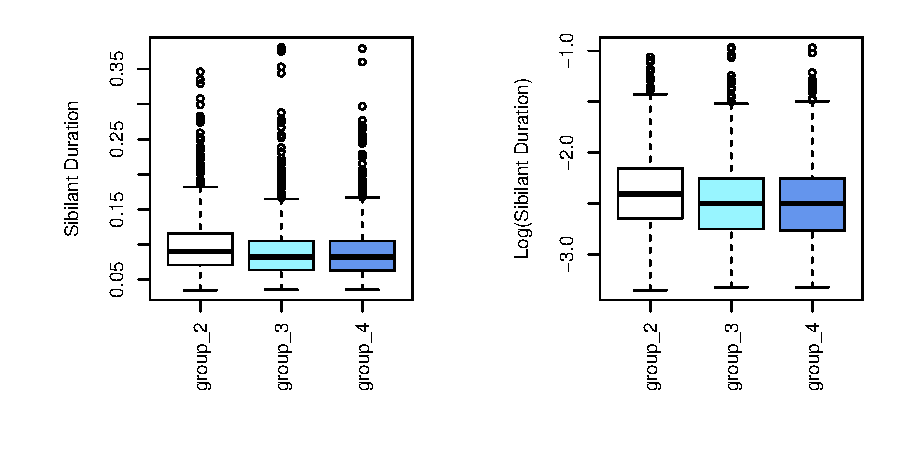
\includegraphics{prelim-059}
      \end{center}
    \end{minipage}
    \caption{Sibilant Duration by Age Group}
    \label{fig:sib.dur.by.age}
  \end{center}
\end{figure}

While the difference between age groups is harder to see with the
significant right skew in Sibilant Duration, it becomes more distinct with
the log-transformation (Figure \ref{fig:sib.dur.by.age}).

In Figure \ref{fig:sib.dur.by.sib}, The interaction between following
segments and standard pronunciations is explored.
For each type of following segment, [s]'s have longer durations than
[z]'s.  Regardless of standard pronunciation, sibilants that precede
pauses are longer than sibilants that precede vowels and consonants,
and there is a lot more variability for these sibilants.  There is
less of a difference (and more variability) between the standard
pronunciations that precede  pauses than for segments that precede
consonants or vowels, which is a good visualization of
the interaction.


\begin{figure}[h!]
  \begin{center}
    \begin{minipage}[t]{0.8\linewidth}
      \begin{center}
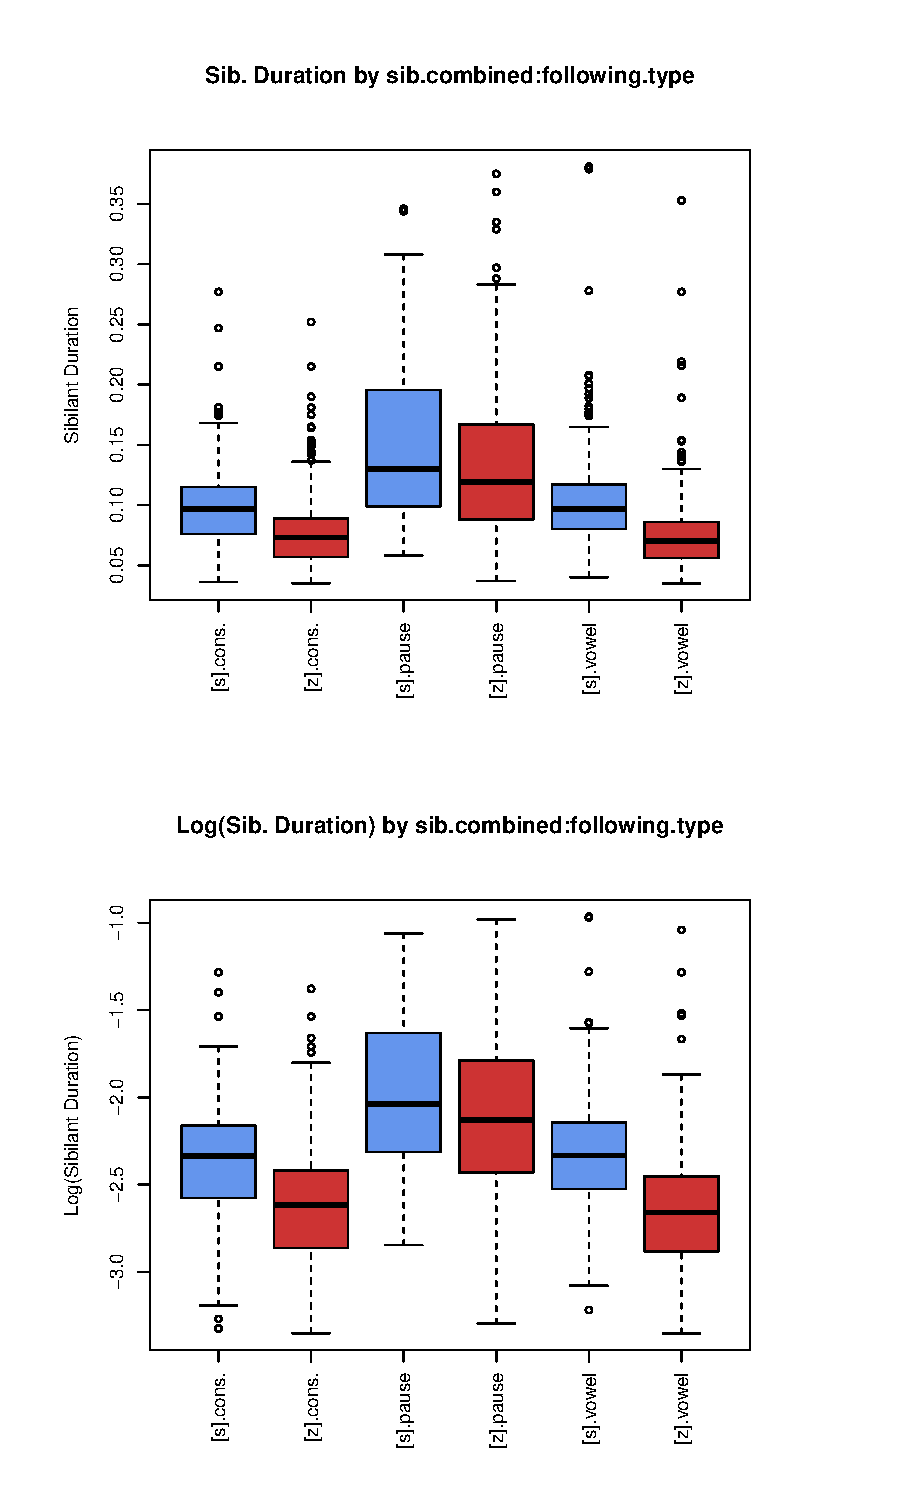
\includegraphics{prelim-061}
      \end{center}
    \end{minipage}
    \caption{Sibilant Duration by Standard Pronunciation and Following Segment}
    \label{fig:sib.dur.by.sib}
  \end{center}
\end{figure}

\begin{figure}[h!]
  \begin{center}
    \begin{minipage}[t]{\linewidth}
      \begin{center}
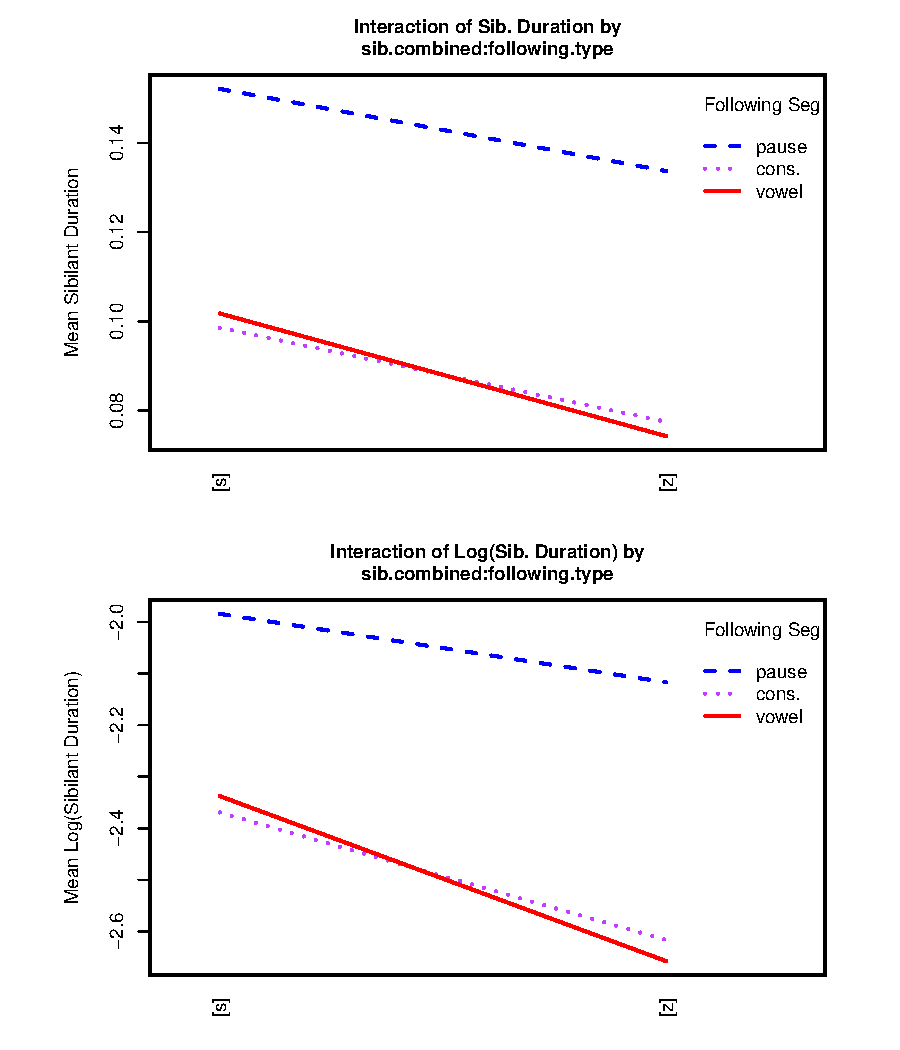
\includegraphics{prelim-063}
      \end{center}
    \end{minipage}
    \caption{Interaction Profiles of Sibilant Duration by\\ Standard Pronunciation
      and Following Segment}
    \label{fig:sib.dur.int}
  \end{center}
\end{figure}
Another visual representation of the interaction is, as its name would
suggest, the Interaction Profile Plot (Figure \ref{fig:sib.dur.int}).  Here,
each line represents the drop in the mean of
Sibilant Duration from [s] to [z] for each of the following segment
types.  Since Sibilant Duration is not significantly different for
following consonants and vowels, the lines overlap, and for
following pauses the line is  much higher.  The interactions are evident
by the different slopes of the lines, with the slope for
following pauses being shallower than the slope for following consonants
(while there is an interaction for vowels, it is insignificant in the
model).
\newpage
For all of these plots, the differences between groups, while they
exist in the untransformed data, become more
distinct when the log-transformation is used.  This is a good demonstration
of the transformation's utility when working with highly skewed data.

\subsection*{Preceding Segment Duration}
\addcontentsline{toc}{subsection}{Preceding Segment Duration}
Preceding Segment Duration will be modeled using a Gamma Generalized Linear
Mixed Model.

\subsection*{Center of Gravity}
\addcontentsline{toc}{subsection}{Center of Gravity}
Center of Gravity will be modeled using a Linear Mixed Model with no
transformation.  Again, the filtered middle 60\% is the best measure
to use.

\subsection*{Percent Voicelessness}
\addcontentsline{toc}{subsection}{Percent Voicelessness}
The best model for Percent Voicelessness still needs to be explored
further.  There are packages that implement Multilevel Beta Regression
in CRAN which are worth looking at.

%%%%%%%%%%%%%%%%%%%%%%%%%%%%%%%%%%%%%%%%%%%%%%%%%%%%%%%%%%%%%%%%%%%%%%%%%%%%%%%%
%%%%%%%%%%%%%%%%%%%%%%%%%%%%%%%%%%%%%%%%%%%%%%%%%%%%%%%%%%%%%%%%%%%%%%%%%%%%%%%%
%%%%%%%%%%%%%%%%%%%%%%%%%%%%%%%%%%%%%%%%%%%%%%%%%%%%%%%%%%%%%%%%%%%%%%%%%%%%%%%%
%%%%%%%%%%%%%%%%%%%%%%%%%%%%%%%%%%%%%%%%%%%%%%%%%%%%%%%%%%%%%%%%%%%%%%%%%%%%%%%%

\newpage
\begin{center} {\bf\huge Appendices} \end{center}
\renewcommand{\thesection}{A.\arabic{section}}
\setcounter{section}{0}
\setcounter{page}{1}
\pagenumbering{roman}
\addcontentsline{toc}{section}{Appendices}
\section{ Variable Definitions}
\label{a:vardef}
\LTXtable{\linewidth}{table.tex}

%%%%%%%%%%%%%%%%%%%%%%%%%%%%%%%%%%%%%%%%%%%%%%%%%%%%%%%%%%%%%%%%%%%%%%%%%%%%%%%%
%%%%%%%%%%%%%%%%%%%%%%%%%%%%%%%%%%%%%%%%%%%%%%%%%%%%%%%%%%%%%%%%%%%%%%%%%%%%%%%%
%%%%%%%%%%%%%%%%%%%%%%%%%%%%%%%%%%%%%%%%%%%%%%%%%%%%%%%%%%%%%%%%%%%%%%%%%%%%%%%%
%%%%%%%%%%%%%%%%%%%%%%%%%%%%%%%%%%%%%%%%%%%%%%%%%%%%%%%%%%%%%%%%%%%%%%%%%%%%%%%%
\newpage
\section{ Code}
\renewcommand{\thesubsection}{\thesection.\alph{subsection}}
\subsection{ Data Shaping}
\begin{Schunk}
\begin{Soutput}
> ## read in main data file
> dat <- read.csv("./data/s_z_final.csv", header=T, na.strings=c("--undefined--", ""))

> ## read in the subsets
> csv.files <- list.files("./data")

> csv.files <- csv.files[!grepl("^[s_z|G234]", csv.files)]

> csv.names <- unlist(strsplit(csv.files, ".csv"))  ##just to have for reference.

> for(file in csv.files){
+     f.name <- strsplit(file, ".csv")[[1]]
+     assign(f.name, read.csv(paste("./data/", file, sep=""), header=T,
+                              na.strings=c("--undefined--", "")))
+ }

> ## Verify that dimensions of subsets match with dimensions of
> ## full data set, just to be safe.
> dim.mat <- t(sapply(csv.names, FUN=function(X) dim(eval(parse(text=X)))))

> sum(dim.mat[,1])/2 == nrow(dat)
[1] TRUE

> table(dim.mat[,2] == ncol(dat))[1]
TRUE
  12

> ## get approx. ages
> dat$age_group <- dat$age

> dat$age <- 2005 - dat$birth_year

> #### Investigate outlier in prec_segment_dur
> (max.dur <- max(dat$prec_segment_dur))
[1] 23.927

> max.ind <- which.max(dat$prec_segment_dur)

> dat$prec_segment_end[max.ind] - dat$prec_segment_start[max.ind]
[1] 23.926

> dat$prec_segment[max.ind]
[1] e
Levels: ^ ! ) @ a A b d e E f g i I j k l m n N o p P r t th u U v w W Y

> ## A 24sec 'e' doesn't make sense and not an obvious arithmetic error. NA it.
> dat$prec_segment_dur[which.max(dat$prec_segment_dur)] <- NA

> #### create a new column for if a token is internal or external
> dat$sib.location <- factor(ifelse(grepl("p|w", dat$sibilant),
+                                   "internal", "word-final"))

> #### create a new column for if sibilant is [s] or [z], regardless of location
> dat$sib.combined <- factor(ifelse(grepl("s|p", dat$sibilant), "[s]", "[z]"))

> #### create look-up tables to find _seg.types
> seg.cons <- c(unique(unlist(lapply(csv.names[grep("PreCon$",csv.names)],
+                      FUN=function(X) levels(eval(parse(text=X))$prec_segment)))),
+                      "ch", "d3", "h", "H", "s", "TH")

> seg.vowels <- unique(unlist(lapply(csv.names[grep("PreVowel$", csv.names)],
+                      FUN=function(X) levels(eval(parse(text=X))$prec_segment))))

> seg.type <- as.list(c(rep("vowel", length(seg.vowels)),
+                     rep("cons.", length(seg.cons)),
+                     "pause"))

> names(seg.type) <- as.list(c(seg.vowels, seg.cons, "#"))

> ## create cols for _segment.types, ignoring NA rows
> dat$prec_segment.type <- as.factor(sapply(dat$prec_segment,
+                                    FUN=function(X) seg.type[[X]]))

> inds.foll <- !is.na(dat$following_segment)

> dat$following_segment.type[inds.foll] <- sapply(as.character(
+         dat$following_segment[inds.foll]), FUN=function(X) seg.type[[X]])

> dat$following_segment.type <- as.factor(dat$following_segment.type)

> #### NA weird data in morphological_standing for now
> summary(dat$morphological_standing)
  first  first   second second    third
   1326       1    1556       1     235

> ## nuke whitespaces
> morpho <- as.character(dat$morphological_standing)

> morpho <- sapply(dat$morphological_standing,
+                  FUN = function(X) sub("[[:blank:]]*$", "", X))

> ## fix obvious typo
> #morpho[which(morpho=="secong")] <- "second"  ##fixed in data
> ## get rid of anything not first, second, or third
> dat$morphological_standing <- factor(ifelse(grepl("first|second|third", morpho),
+                                             morpho, NA))

> summary(dat$morphological_standing)
 first second  third
  1327   1557    235
\end{Soutput}
\end{Schunk}

\subsection{ Independant Variable Plots}
\setlength{\parindent}{0pt}
Figure \ref{fig:token_count} (page \pageref{fig:token_count}):
\begin{Schunk}
\begin{Sinput}
> barplot(sort(as.vector(table(dat$speaker))))
> abline(h=round(mean(table(dat$speaker))), col="red", lwd=3)
\end{Sinput}
\end{Schunk}

Figure \ref{fig:social_by_token} (page \pageref{fig:social_by_token}):
\begin{Schunk}
\begin{Sinput}
> social <- dat[,c(1:5, 7:9, 36)]
> par(mfrow=c(1,7), cex.axis=2, las=3, cex.main=2, mai=c(1.5, .5, .5, .25))
> barplot(table(social$ethnicity), main="Ethnicity")
> barplot(table(social$college), main="College")
> barplot(table(social$region), main="Region")
> barplot(table(social$sex), main="Sex")
> barplot(table(social$rurality), main="Rurality")
> barplot(table(social$class), main="Class")
> barplot(table(social$age_group), main="Age Group")
\end{Sinput}
\end{Schunk}

Figure \ref{fig:social_by_speaker} (page \pageref{fig:social_by_speaker}):
\begin{Schunk}
\begin{Sinput}
> library(plyr)
> social.speaker <- ddply(social, ~ speaker, count)[,-10]
> par(mfrow=c(1,7), cex.axis=2, las=3, cex.main=2, mai=c(1.5, .5, .5, .25))
> barplot(table(social.speaker$ethnicity), main="Ethnicity")
> barplot(table(social.speaker$college), main="College")
> barplot(table(social.speaker$region), main="Region")
> barplot(table(social.speaker$sex), main="Sex")
> barplot(table(social.speaker$rurality), main="Rurality")
> barplot(table(social.speaker$class), main="Class")
> barplot(table(social.speaker$age_group), main="Age Group")
\end{Sinput}
\end{Schunk}

Figure \ref{fig:age_by_speaker} (page \pageref{fig:age_by_speaker}):
\begin{Schunk}
\begin{Sinput}
> par(mfrow=c(1,1), mai=c(.5, 1, .5, .5))
> hist(social.speaker$age, col="darkgrey", xlab="Age",
+      main="", cex.axis=2, cex.lab=2)
\end{Sinput}
\end{Schunk}

Figure \ref{fig:morpho} (page \pageref{fig:morpho}):
\begin{Schunk}
\begin{Sinput}
> par(cex.axis=2, cex.lab=2, cex.main=2, mai=c(.5, .5, 1, 0))
> barplot(summary(dat$morphological_standing),  main="Morphological Standing")
> par(cex.axis=2, cex.lab=2, cex.main=2)
> barplot(summary(dat$sib.location), main="Sibilant Location")
\end{Sinput}
\end{Schunk}


Figure \ref{fig:phono} (page \pageref{fig:phono}):
\begin{Schunk}
\begin{Sinput}
> par(mfrow=c(1,3))
> barplot(summary(dat$prec_segment.type), main="Preceding\n Segment Type")
> barplot(summary(dat$following_segment.type), main="Following\n Segment Type", las=3)
> barplot(summary(dat$sib.combined), main="Standard Pronunciation")
\end{Sinput}
\end{Schunk}

Figure \ref{fig:sib.intensity} (page \pageref{fig:sib.intensity}):
\begin{Schunk}
\begin{Sinput}
> par(mfrow=c(1, 3), cex=.75, cex.main=1)
> hist(dat$sib_intensity05, main="Sib. Intensity 5%",
+      xlab="Intensity", col="darkgrey", freq=FALSE, ylim=c(0, 0.045))
> lines(density(dat$sib_intensity05), col="red", lwd=2)
> hist(dat$sib_intensity25, main="Sib. Intensity 25%",
+      xlab="Intensity", col="darkgrey", freq=FALSE, ylim=c(0, 0.045))
> lines(density(dat$sib_intensity25), col="red", lwd=2)
> hist(dat$sib_intensity50, main="Sib. Intensity 50%",
+      xlab="Intensity", col="darkgrey", freq=FALSE, ylim=c(0, 0.045))
> lines(density(dat$sib_intensity50), col="red", lwd=2)
\end{Sinput}
\end{Schunk}

Figure \ref{fig:prec.intensity} (page \pageref{fig:prec.intensity}):
\begin{Schunk}
\begin{Sinput}
> par(mfrow=c(1, 3), cex=.75, cex.main=1)
> hist(dat$prec_segment_intensity05, main="Prec. Segment Intensity 5%",
+      xlab="Intensity", col="darkgrey", freq=FALSE)
> lines(density(dat$prec_segment_intensity05), col="red", lwd=2)
> hist(dat$prec_segment_intensity25, main="Prec. Segment Intensity 25%",
+      xlab="Intensity", col="darkgrey", freq=FALSE)
> lines(density(dat$prec_segment_intensity25), col="red", lwd=2)
> hist(dat$prec_segment_intensity50, main="Prec. Segment Intensity 50%",
+      xlab="Intensity", col="darkgrey", freq=FALSE)
> lines(density(dat$prec_segment_intensity50), col="red", lwd=2)
\end{Sinput}
\end{Schunk}
%%%%%%%%%%%%%%%%%%%%%%%%%%%%%%%%%%%%%%%%%%%%%%%%%%%%%%%%%%%%%%%%%%%%%%%%%%%%%%%%
%%%%%%%%%%%%%%%%%%%%%%%%%%%%%%%%%%%%%%%%%%%%%%%%%%%%%%%%%%%%%%%%%%%%%%%%%%%%%%%%
%%%%%%%%%%%%%%%%%%%%%%%%%%%%%%%%%%%%%%%%%%%%%%%%%%%%%%%%%%%%%%%%%%%%%%%%%%%%%%%%
%%%%%%%%%%%%%%%%%%%%%%%%%%%%%%%%%%%%%%%%%%%%%%%%%%%%%%%%%%%%%%%%%%%%%%%%%%%%%%%%
\subsection{ Dependant Variable Plots}
Figure \ref{fig:sib_dur_hist} (page \pageref{fig:sib_dur_hist}):
\begin{Schunk}
\begin{Sinput}
> par(cex=1, cex.lab=2, cex.main=2, cex.axis=2, mai=c(1, 1, 0, .5))
> hist(dat$sib_dur, freq=FALSE, xlab="Duration (sec)", main="",
+      ylim=c(0, 13), col="darkgrey")
> lines(density(dat$sib_dur), col="red", lwd=3)
\end{Sinput}
\end{Schunk}

Figure \ref{fig:sib_dur_qq} (page \pageref{fig:sib_dur_qq}):
\begin{Schunk}
\begin{Sinput}
> library(MASS); library(car)
> par(mfrow=c(1, 3), cex=.5, cex.main=1.5, cex.lab= 1.5, cex.axis=1,
+     mai=c(.5, .65, .5, 0))
> qqPlot(dat$sib_dur, main="Normal Q-Q", ylab="Sibilant Duration", lwd=1)
> qqPlot(log(dat$sib_dur), main="Lognormal Q-Q", ylab="Log(Sibilant Duration)", lwd=1)
> gamma.coef <- round(fitdistr(dat$sib_dur, "gamma")[[1]], 3)
> qqPlot(dat$sib_dur, "gamma", shape=gamma.coef[1], rate=gamma.coef[2],
+        main="Gamma Q-Q", ylab="Sibilant Duration", lwd=1)
\end{Sinput}
\end{Schunk}

Figure \ref{fig:prec_dur_hist} (page \pageref{fig:prec_dur_hist}):
\begin{Schunk}
\begin{Sinput}
> par(cex=1, cex.lab=2, cex.main=2, cex.axis=2, mai=c(1, 1, 0, .5))
> hist(dat$prec_segment_dur, freq=FALSE, xlab="Duration (sec)", main="",
+      ylim=c(0, 9), col="darkgrey")
> lines(density(dat$prec_segment_dur[!is.na(dat$prec_segment_dur)]),
+       col="red", lwd=3)
\end{Sinput}
\end{Schunk}

Figure \ref{fig:prec_dur_qq} (page \pageref{fig:prec_dur_qq}):
\begin{Schunk}
\begin{Sinput}
> par(mfrow=c(1, 3), cex=.5, cex.main=1.5, cex.lab= 1.5, cex.axis=1,
+     mai=c(.5, .65, .5, 0))
> qqPlot(dat$prec_segment_dur, main="Normal Q-Q", ylab="Duration", lwd=1)
> qqPlot(log(dat$prec_segment_dur), main="Lognormal Q-Q", ylab="Log(Duration)", lwd=1)
> gamma.coef <- round(fitdistr(dat$prec_segment_dur[!is.na(dat$prec_segment_dur)],
+                              "gamma")[[1]], 3)
> qqPlot(dat$prec_segment_dur, "gamma", shape=gamma.coef[1], rate=gamma.coef[2],
+        main="Gamma Q-Q", ylab="Duration", lwd=1)
\end{Sinput}
\end{Schunk}

Figure \ref{fig:cog_hist} (page \pageref{fig:cog_hist}):
\begin{Schunk}
\begin{Sinput}
> par(mfrow=c(2,2), cex=.5, cex.main=1.5, cex.lab= 1.5, cex.axis=1,
+     mai=c(.5, .5, .25, 0))
> hist(dat$sib_COG_full, xlab="CoG", main="Full CoG", freq=FALSE, col="darkgrey",
+      ylim=c(0, 5e-4))
> lines(density(dat$sib_COG_full), col="red")
> hist(dat$sib_COG_60, xlab="CoG", main="60% CoG", freq=FALSE, col="darkgrey")
> lines(density(dat$sib_COG_60), col="red")
> hist(dat$sib_COG_filtered, xlab="CoG", main="Filtered CoG", freq=FALSE,
+      col="darkgrey")
> lines(density(dat$sib_COG_filtered), col="red")
> hist(dat$sib_COG_60_filtered, xlab="CoG", main="Filtered 60% CoG", freq=FALSE,
+      col="darkgrey")
> lines(density(dat$sib_COG_60_filtered), col="red")
\end{Sinput}
\end{Schunk}

Figure \ref{fig:cog_qq} (page \pageref{fig:cog_qq}):
\begin{Schunk}
\begin{Sinput}
> par(mfrow=c(1,1), cex=1, cex.lab=1.5, cex.main=1.5, cex.axis=1,
+     mai=c(1, 1, 0, 0))
> qqPlot(dat$sib_COG_60_filtered, ylab="CoG")
\end{Sinput}
\end{Schunk}

Figure \ref{fig:vls_hist} (page \pageref{fig:vls_hist}):
\begin{Schunk}
\begin{Sinput}
> par(cex=1, cex.lab=1.25, cex.main=1.5)
> hist(dat$vls_percent, freq=FALSE, xlab="Voicelessness (%)",
+      col="darkgrey", main="")
> lines(density(dat$vls_percent), col="red", lwd=2)
\end{Sinput}
\end{Schunk}

Figure \ref{fig:vls_qq} (page \pageref{fig:vls_qq}):
\begin{Schunk}
\begin{Sinput}
> qqPlot(dat$vls_percent, "beta", shape1=0.5, shape2=0.35,
+        ylab="Voicelessness (%)")
\end{Sinput}
\end{Schunk}

\subsection{ Analysis}
\renewcommand{\thesubsubsection}{\thesubsection.\roman{subsubsection}}
\subsubsection{ Sibilant Duration}
\begin{Schunk}
\begin{Sinput}
> ######### Define a print function for model summaries that
> ######### typesets things better
> pretty.summary.print <- function(mod.sum){
+     cat("\\begingroup
+         \\catcode\`_=\\active
+         \\gdef\\works{
+            \\catcode\`_=\\active
+            \\def_{\\textunderscore\\-}%
+         }")
+     cat("\\texttt{")
+     cat(mod.sum$methTitle, "\\newline ")
+     cat("Formula:\\newline ")
+     print(mod.sum$call)
+     cat("\\newline\\newline REML at convergence: ", mod.sum$AICtab, "\\newline ")
+     cat("\\newline\ Random Effects:\\newline ")
+     retab <- data.frame(mod.sum$varcor, stringsAsFactors=FALSE)[,-3]
+     colnames(retab) <- c("Groups", "Name", "Variance", "St.Dev.")
+     retab$Name[3] <- ""
+     retab <- xtable(retab)
+     print(retab, floating=FALSE, include.rownames=FALSE)
+     cat("\\newline Number of obs: ", length(residuals(mod.sum)),
+         ", groups: ", "word, ", mod.sum$ngrps[1], "; speaker, ",
+         mod.sum$ngrps[2], "\\newline ", sep="")
+     cat("\\newline Fixed Effects:\\newline ")
+     coefs <- xtable(mod.sum$coef, digits=3)
+     print(coefs, floating=FALSE)
+     cat("}\\endgroup\\newline")
+ }
> ######### Rename and subset data better for analysis
> ######### & create the basis model
> library(xtable)
> library(lme4, quietly=TRUE)
> library(lmerTest, quietly=TRUE, warn.conflicts=FALSE)
> #### Get a data frame with only the variables under consideration
> dat2 <- dat[,c(1:4, 7:9, 11:12, 16:17, 21:24, 28, 29:34, 36:40)]
> colnames(dat2)[6] <- "social.class" #to avoid confusion with function class()
> #### Shorten names for narrower printing
> colnames(dat2)[9] <- "morph.standing"
> colnames(dat2)[12] <- "sib.cog"
> colnames(dat2)[17:19] <- paste(rep("prec.int", 3),
+                                c("05", "25", "50"), sep="")
> colnames(dat2)[20:22] <- paste(rep("prec.pitch", 3),
+                                c("05", "25", "50"), sep="")
> colnames(dat2)[26:27] <- c("prec.type", "following.type")
> #### scale COG & intensities
> dat2$sib.cog <- scale(dat2$sib.cog)
> dat2[,17:19] <- scale(dat2[,17:19])
> dat2[,20:22] <- scale(dat2[,20:22])
> ## omit rows w/ NAs so all models have same number of observations
> dat2 <- na.omit(dat2)
> #### get base model
> sib.dur.0 <- lmer(log(sib_dur) ~ prec_segment_dur + sib.cog
+                  + vls_percent + (1|word) + (1|speaker), dat2)
> s0 <- summary(sib.dur.0)
> pretty.summary.print(s0)
> ######### Get things prepped for step function & use it for low level vars.
> source("forward.lmer.R")
> #### forward.lmer only takes variable names, not a formula for upper, which is
> #### rather inconvenient.  Create vectors of variable names & interactions:
> terms <- list(
+     soc = colnames(dat2)[c(2:7, 23)],
+     morpho = colnames(dat2)[c(9,24)],
+     phonol = colnames(dat2)[25:27],
+     phonetic = colnames(dat2)[c(13:15, 17:22)]
+ )
> #### get interactions
> interact <- function(vars){
+     interact <- vars
+     for(i in 1:(length(vars)-1)){
+         for(j in (i+1):length(vars)){
+             interact <- append(interact, paste(vars[i], vars[j], sep=":"))
+         }
+     }
+     interact
+ }
> terms <- lapply(terms, interact)
> #### start modeling.  huzzah.  may take a while.
> ## time <- system.time(sib.dur.1 <- forward.lmer(sib.dur.0,
> ##                                   blocks=terms$phonetic,
> ##                                   max.iter = length(terms$phonetic),
> ##                                   sig.level=0.05, print.log=FALSE))
> s1 <- summary(sib.dur.1)
> #### re-run model w/ lmerTest to we can can p-vals
> s1 <- summary(sib.dur.1 <- lmerTest::lmer(s1$call$formula, dat2))
> pretty.summary.print(s1)
> cat("\\newline\\newline\\texttt{Selection completed in",
+     round(time[3]/60, 1), "minutes.}\\newline\\newline")
> ######### add pitch05, check fit, & print new coef tab
> sib.dur.1.1 <- update(sib.dur.1, . ~ . + prec.pitch05)
> print(xtable(anova(sib.dur.1.1, sib.dur.1)), table.placement="h!")
> sib.dur.1.1 <- lmer(summary(sib.dur.1.1)$call$formula, dat2)
> pretty.summary.print(summary(sib.dur.1.1))
> ######### Start selecting high level terms
> ## time2 <- system.time(sib.dur.2 <- forward.lmer(sib.dur.1.1,
> ##                                     blocks=c(terms$morpho, terms$soc, terms$phono,
> ##                                              "sib.combined:sib.location"),
> ##                                     max.iter = length(c(terms$morpho, terms$soc,
> ##                                                       terms$phono)) + 1,
> ##                                     sig.level=0.05, print.log=FALSE))
> s2 <- summary(sib.dur.2)
> #### re-run model w/ lmerTest to we can get can p-vals
> s2 <- summary(sib.dur.2 <- lmerTest::lmer(s2$call$formula, dat2))
> pretty.summary.print(s2)
> cat("\\newline\\newline\\texttt{Selection completed in",
+     round(time2[3]/60, 2), "minutes.}\\newline\\newline")
> #### Manually add following.type
> sib.dur.2.0 <- update(sib.dur.2, .~. + following.type + sib.combined)
> #### Manually drop prec.int25, verify, & print new coef tab
> sib.dur.2.0 <- lmer(summary(sib.dur.2.0)$call$formula, dat2)
> pretty.summary.print(summary(sib.dur.2.0))
> cat("\\newline\\newline")
> sib.dur.2.1 <- lmer(summary(sib.dur.2.1)$call$formula, dat2)
> pretty.summary.print(summary(sib.dur.2.1))
> ######## Compare grouping strategies
> sib.dur.3 <- update(sib.dur.2.1, . ~ . - (1|word) - (1|speaker) + (1|speaker/word))
> sib.dur.3 <- lmerTest::lmer(summary(sib.dur.3)$call$formula, dat2)
> pretty.summary.print(summary(sib.dur.3))
> cat("\\newline\\newline")
> a <- anova(sib.dur.2.1, sib.dur.3)
> rownames(a) <- c("Crossed", "Nested")
> print(xtable(a), table.position="h!")
> ######## Get a pretty coefficient table for reference
> print(xtable(summary(sib.dur.3)$coef,
+              caption="Coefficients of Final Sibilant Duration Model",
+              label="tab:sib.dur", digits=3), table.placement="h!")
\end{Sinput}
\end{Schunk}
{\bf Exploratory Plots}\\
Figure \ref{fig:sib.dur.res} (page \pageref{fig:sib.dur.res}):
\begin{Schunk}
\begin{Sinput}
> par(mfrow=c(1,2), mai=c(.75, .75, .5, 0), cex=.75, cex.main=1, cex.lab=1)
> qqPlot(residuals(sib.dur.3), main="Normal Q-Q", ylab="Residual")
> plot(1:length(residuals(sib.dur.3)), residuals(sib.dur.3),
+      xlab="Index", ylab="Residual", main="Residual by Index")
> abline(h=0, col="red", lwd=2)
\end{Sinput}
\end{Schunk}

Figure \ref{fig:sib.dur.by.age} (page \pageref{fig:sib.dur.by.age}):
\begin{Schunk}
\begin{Sinput}
> par(mfrow=c(1,2), las=3, mai=c(1, 1, .25, .25), cex=.75, cex.main=1, cex.lab=1)
> with(dat2, boxplot(sib_dur ~ age_group,
+      ylab="Sibilant Duration", xlab="",
+      col=c("white", "cadetblue1", "cornflowerblue",
+      main="Sib. Duration by Age Group")))
> with(dat2, boxplot(log(sib_dur) ~ age_group,
+      ylab="Log(Sibilant Duration)", xlab="",
+      col=c("white", "cadetblue1", "cornflowerblue",
+      main="Log(Sib. Duration) by Age Group")))
\end{Sinput}
\end{Schunk}

Figure \ref{fig:sib.dur.by.sib} (page \pageref{fig:sib.dur.by.sib}):
\begin{Schunk}
\begin{Sinput}
> par(mfrow=c(2,1), las=3, cex=.75, cex.main=1.25, cex.lab=1,
+     mai=c(1, 1, 1, 1))
> with(dat2, boxplot(sib_dur ~ sib.combined*following.type,
+                    ylab="Sibilant Duration",
+                    col=c("cornflowerblue", "brown3"),
+                    main="Sib. Duration by sib.combined:following.type"))
> with(dat2, boxplot(log(sib_dur) ~ sib.combined*following.type,
+                    ylab="Log(Sibilant Duration)",
+                    main="Log(Sib. Duration) by sib.combined:following.type",
+                    col=c("cornflowerblue", "brown3")))
\end{Sinput}
\end{Schunk}

Figure \ref{fig:sib.dur.int} (page \pageref{fig:sib.dur.int}):
\begin{Schunk}
\begin{Sinput}
> par(mfrow=c(2,1), las=3, cex=.75, cex.main=1, cex.lab=1,
+     mai=c(.5, 1, .5, .5), lwd=2)
> interaction.plot(dat2$sib.combined, dat2$following.type, dat2$sib_dur,
+                  lwd=2, col=c("darkorchid1", "blue", "red"),
+                  xlab="",
+                  ylab="Mean Sibilant Duration",
+                  main="Interaction of Sib. Duration by\nsib.combined:following.type",
+                  trace.label="Following Seg.", xpd=TRUE)
> interaction.plot(dat2$sib.combined, dat2$following.type, log(dat2$sib_dur),
+                  lwd=2, col=c("darkorchid1", "blue", "red"),
+                  xlab="",
+                  ylab="Mean Log(Sibilant Duration)",
+                  main="Interaction of Log(Sib. Duration) by\nsib.combined:following.type",
+                  trace.label="Following Seg.", xpd=TRUE)
\end{Sinput}
\end{Schunk}

%%%%%%%%%%%%%%%%%%%%%%%%%%%%%%%%%%%%%%%%%%%%%%%%%%%%%%%%%%%%%%%%%%%%%%%%%%%%%%%%
%%%%%%%%%%%%%%%%%%%%%%%%%%%%%%%%%%%%%%%%%%%%%%%%%%%%%%%%%%%%%%%%%%%%%%%%%%%%%%%%
%%%%%%%%%%%%%%%%%%%%%%%%%%%%%%%%%%%%%%%%%%%%%%%%%%%%%%%%%%%%%%%%%%%%%%%%%%%%%%%%
%%%%%%%%%%%%%%%%%%%%%%%%%%%%%%%%%%%%%%%%%%%%%%%%%%%%%%%%%%%%%%%%%%%%%%%%%%%%%%%%
\subsection{ Word Frequencies}
\label{a:res}
\begin{Schunk}
\begin{Sinput}
> library(lme4)
> (n.unique.words <- length(table(dat$word)))
\end{Sinput}
\begin{Soutput}
[1] 1295
\end{Soutput}
\begin{Sinput}
> (n.hapax <- length(table(dat$word)[table(dat$word) == 1]))
\end{Sinput}
\begin{Soutput}
[1] 790
\end{Soutput}
\end{Schunk}
\begin{center}
  \begin{minipage}[t]{\linewidth}
    \begin{center}
\begin{Schunk}
\begin{Sinput}
> par(mfrow=c(1,2), cex=.75, cex.main=1, cex.lab=1)
> #### Zipf's Law:
> plot(sort(table(dat$word), decreasing=TRUE),
+      main="Word Frequency by Index",
+      ylab="Frequency", pch=20)
> ## Log-Log should be roughly linear:
> plot(log(sort(table(dat$word), decreasing=TRUE)), log(1:n.unique.words),
+      main="Word Freq. by Index (Log-Log)",
+      xlab="Log(Index)", ylab="Log(Freq.)", pch=20)
> abline(a=6.9, b=-1.5,
+             col="red", lwd=2)
\end{Sinput}
\end{Schunk}
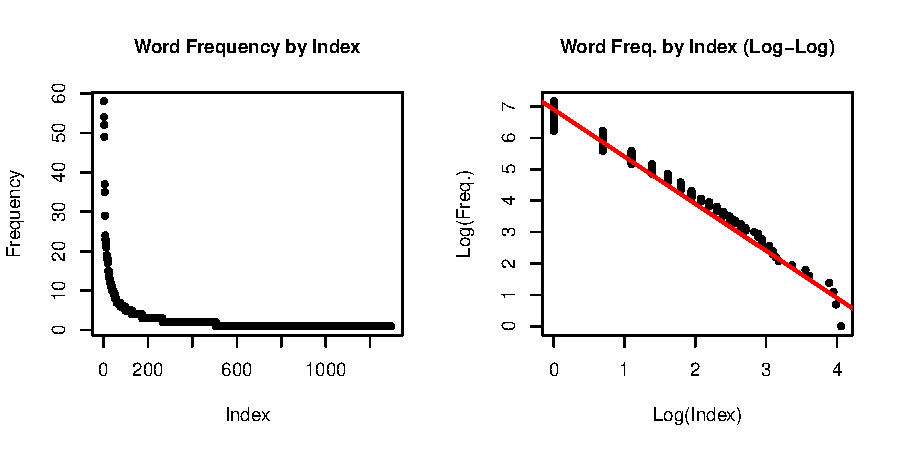
\includegraphics{prelim-087}
    \end{center}
  \end{minipage}
\end{center}
\begin{Schunk}
\begin{Sinput}
> #### Look at words within speaker:
> speaker.word.count <- by(dat$word, dat$speaker, count)
> speaker.word.table <- sapply(speaker.word.count, nrow)
> summary(speaker.word.table)
\end{Sinput}
\begin{Soutput}
   Min. 1st Qu.  Median    Mean 3rd Qu.    Max.
  21.00   36.00   40.00   39.06   42.00   49.00
\end{Soutput}
\begin{Sinput}
> barplot(sort(speaker.word.table), main="Number of Unique Words by Speaker")
> abline(h=mean(speaker.word.table), col="red")
> #### Double check that lmer() gets the same number of unique words and
> #### figure out the number of groups in nested structure
> summary(lmer(sib_dur ~ (1|speaker) + (1|word), dat))$ngrps  #crossed
\end{Sinput}
\begin{Soutput}
   word speaker
   1295      67
\end{Soutput}
\begin{Sinput}
> summary(lmer(sib_dur ~ (1|speaker/word), dat))$ngrps  #nested
\end{Sinput}
\begin{Soutput}
word:speaker      speaker
        2617           67
\end{Soutput}
\end{Schunk}

\end{document}
